\documentclass[a4paper,danish,11pt]{article}

% Skrifttype
\usepackage{lmodern}

% Understøttelse af dansk
\usepackage{babel}
\usepackage[utf8]{inputenc}
\usepackage[T1]{fontenc}

% Matematik-udvidelser
\usepackage{amsmath}
\usepackage{amssymb}
\usepackage{amsthm}

% Graphics-udvidelser
\usepackage{graphicx}

% Hyperlink-udvidelser
\usepackage{hyperref}

% Nye kommandoer
\newcommand{\HRule}{\rule{\linewidth}{0.5mm}}

% Theorem udvidelser
\theoremstyle{plain}
\newtheorem{lemma}{Lemma} 
\newtheorem{pro}{Proof}
\newtheorem{dipro}[pro]{Disproof}

% Source code extensions
\usepackage{listings}
% example {\lstset{style=JavaCode}\begin{lstlisting}public void do() { }\end{lstlisting}}
% remember to enlose, to make \lstset arguments, "`private"'
\usepackage{xcolor}
% JavaCode Listing Style
% Author: Michael Dahl <micdah@gmail.com>
% Defines a nice java code style, for usage with listings

\definecolor{lstJavaCodeBasic}{rgb}{0,0,0}
\definecolor{lstJavaCodeComment}{rgb}{0.5,0.5,0.5}
\definecolor{lstJavaCodeComment2}{rgb}{0.0,0.4,0.5}
\definecolor{lstJavaCodeString}{rgb}{0.0,0.5,0.683}
\definecolor{lstJavaCodeKeyword}{rgb}{0.5,0.0,0.333}
\definecolor{lstJavaCodeNumber}{rgb}{.33,.33,.33}
\definecolor{lstJavaCodeRule}{rgb}{.2,.4,.6}
\lstdefinestyle{JavaCode}{
	language=Java,
	numbers=left,
	stepnumber=1,
	firstnumber=1,
	tabsize=4,
	breaklines=true,
	frame=single,
	frameround=tttt,
	rulecolor=\color{lstJavaCodeRule},
	numberstyle=\color{lstJavaCodeNumber}\tiny,
	basicstyle=\color{lstJavaCodeBasic}\sffamily\scriptsize,
	commentstyle=\color{lstJavaCodeComment}\sffamily\textit,
	morecomment=[s][\color{lstJavaCodeComment2}\sffamily\textit]{/**}{*/},
	stringstyle=\color{lstJavaCodeString},
	keywordstyle=\color{lstJavaCodeKeyword}\sffamily\textbf
}

\title{dKS Noter}
\author{Michael Lind Mortensen, illio}
\begin{document}
\maketitle
\thispagestyle{empty}

\newpage

\tableofcontents

\newpage
 
\section{P, NP and NPC.}

\subsection{Disposition}

\begin{enumerate}
 \item \textbf{Def. Problemer, Sprog, Encoding \& Stand-in Sprog}
    \subitem Def. Beslutningsproblem
    \subitem Def. Sprog
    \subitem Encoding
    \subitem Stand-in sprog
    \subitem Optimization Stand-ins
 \item \textbf{Def. P, NP, NP-hard \& NPC}
    \subitem  Tegn!
 \item \textbf{Def. Polynomial time computable maps}
 \item \textbf{Def. Reduktioner}
    \subitem  Proposition 3: Transitivitet (med bevis)
    \subitem  Proposition 4: Nedadgående lukkethed af P (uden bevis)
 \item \textbf{Lemma 7:} \textit{Hvis $L_1 \in$ NP-hard og $L_1 \leq L_2$, så er $L_2 \in$ NP-hard}
    \subitem  Bevis.
 \item \textbf{Proposition 5:} \textit{Lad $L \in$ NP-hard. Hvis $P \neq NP$, så er $L \notin P$.}
    \subitem  Bevis.
 \item \textbf{Proposition 6:} \textit{Hvis $L \in NPC$, så er $L \in P$ hviss. $P=NP$}
    \subitem  Bevis
 \item \textbf{Theorem 9.4:} \textit{INDEPENDENT SET $\in$ NPC}
    \subitem Vis 3SAT $\leq$ INDEPENDENT SET.
\end{enumerate}

\subsection{Emne detaljer}

Følgende afsnit indeholder detaljer om hvert punkt i dispositionen ovenfor (og muligvis flere ting også).

\subsubsection{Def. Problemer, Sprog, Encoding \& Stand-in Sprog}

Lad os starte med lige at få nogle grundlæggende definitioner og koncepter på plads. 

\paragraph{Def. Beslutningsproblem}
~\\
~\\
Vi fokuserer på såkaldte beslutningsproblemer hvor output altid er ''yes`` eller ''no``. Input her er så probleminstanser givet ved binære strenge. Altså strenge over $\left\lbrace 0,1 \right\rbrace$.

\paragraph{Def. Sprog}
~\\
~\\
Et givent problem, kan så modeleres som et sprog $L \subseteq \left\lbrace 0,1 \right\rbrace^*$ hvor medlemmerne af sproget er de instanser for hvilket output er ''yes`` og ikke-medlemmerne er de instanser hvor hvilket output er ''no``.

\paragraph{Encoding}
~\\
~\\
Vi sætter som sagt den ''restriktion`` at input er bitstrenge på $\left\lbrace 0,1 \right\rbrace^*$. Det er dog ikke en reel begrænsning, da reele computere alligevel gør selv samme med alt data gemt derpå. Således kan ethvert ''naturligt`` dataformat encodes som binært, således selv ASCII og UNICODE encodes nemt.
Dog er der selvfølgelig ting som selv en reel computer ikke kan encode korrekt i alle tilfælde, så som reele tal.

\paragraph{Stand-in sprog}
~\\
~\\
Hvis vi har et problem, for hvilket output ikke direkte kan beskrives som ''yes`` eller ''no``, men i stedet bør være en arbitrær bitstreng. Så konstruerer vi i stedet et såkaldt ''stand-in'' sprog. 

Et ``stand-in'' sprog $L_f$ repræsenterer så en given funktion $f: \left\lbrace 0,1 \right\rbrace^* \rightarrow \left\lbrace 0,1 \right\rbrace^*$ således:

\begin{align*}
 L_f &= \left\lbrace \left\langle x, b(j), y \right\rangle | f(x)_j = y \right\rbrace
\end{align*}
Hvor:\\
~\\
$x \in \left\lbrace 0,1 \right\rbrace^*$ \\
$j \in N$ \\
$y \in \left\lbrace 0,1 \right\rbrace$ \\

Og hvor $b(j)$ betyder den binære encodning af $j$. 

Her har vi, at $L_f$ har en effektiv algoritme, hvis og kun hvis, $f$ har det. Man skal så forstå ovenstående som, at output udregnes en bit af gangen.

\paragraph{Optimization Stand-ins}
~\\
~\\
Ligesom for arbitrære funktioner på bitstrenge, så skal vi også kunne modellere optimeringsproblemer. Lad os antage vi har fået følgende beskrivelse af et optimeringsproblem:

\begin{quotation}
 \textbf{OPT:} ``Givet en inputstreng der definerer et sæt mulige løsninger $F$ og en objective funktion $f$, find $x \in F$ der maksimerer $f(x)$''.
\end{quotation}

Dette kan vi så udtrykke som et beslutningsproblem ved blot at lave en lille ændring.

\begin{quotation}
 \textbf{OPT:} ``Givet en inputstreng der definerer $F$, $f$ og en target værdi $v \in Q$, bestem hvorvidt der er en løsning $x \in F$ således $f(x) \geq v$.''.
\end{quotation}

Det er dog ikke en perfekt ``stand-in'', da $L_{OPT}$ f.eks. godt kan være nem at løse uden at $OPT$ er det. Omvendt så hvis $L_{OPT}$ er svær at løse, så ved vi også $OPT$ er det. Det er således ikke muligt at bruge denne form for ``stand-in'' til at vise et givet problem er nemt at løse, men vi kan bruge det til at argumentere for et givent problem er svært.


\subsubsection{Def. P, NP, NP-hard \& NPC}

Lad os nu kigge på de kompleksitetsklasser vi har arbejdet med her i kurset.
\begin{center}
 \includegraphics[bb=0 0 400 400,scale=0.3]{./PNPNPC.png}
 % PNPNPC.png: 1667x1667 pixel, 300dpi, 14.11x14.11 cm, bb=0 0 400 400
\end{center}


\paragraph{P}
~\\
~\\
Kompleksitetsklassen $P$ er formelt defineret således:
\begin{align*}
 P = \left\lbrace L \subseteq \left\lbrace 0,1 \right\rbrace^* | \exists \text{ TM } M_L \text{ der afgører L i polynomiel tid } \right\rbrace
\end{align*}
Altså klassen af beslutningsproblemer der kan blive bestemt af en deterministisk Turing Maskine hvor antallet af ``steps'' maskinen udfører for et givent $x$ maksimalt er $\rho(x)$ for et givent polynomiel $\rho$.\\
 
Intuivit ser vi kompleksitetsklassen $P$ som en klasse for problemer for hvilket vi kender en effektiv løsning. Altså ethvert problem med worst-case kørselstid på formen $O(n^k)$ for et givent $k$.

At worst-case kørseltid på et problem er polynomiel betyder dog ikke reelt at det er et nemt problem (modsat hvad Cobham's Thesis påstår). I hele den analyse ignorerer vi fuldkommen konstanter, samt forventet kørselstid som I mange tilfælde kan få ``sværere'' problemer til at køre bedre end ``nemme'' problemer i $P$.


\paragraph{NP}
~\\
~\\
Kompleksitetsklassen $NP$ er lidt mere kluntet formelt defineret, så vi starter lige med intuitionen først.

Intuitivt kan $NP$ ses som klassen af beslutningsproblemer for hvilket ``yes'' instanserne kan verificeres i polynomiel tid på en deterministisk Turing Maskine. Altså er det komplekse problemer med eksponentiel løbetid, men hvor løsningen til et sådant problem nemt kan verificeres til at være korrekt.\\
~\\
Kompleksitetsklassen $NP$ er formelt defineret således:
\begin{align*}
 NP = \left\lbrace L \subseteq \left\lbrace 0,1 \right\rbrace^* | \exists \rho \in Z[x], L' \in P, \forall x \in \left\lbrace 0,1 \right\rbrace^* : ( x \in L \Leftrightarrow \exists y \in \left\lbrace 0,1 \right\rbrace^* : |y| \leq \rho(|x|) \wedge \left\langle x,y \right\rangle \in L') \right\rbrace
\end{align*}
Definitionen skal forståes således: Vi har et sprog $L' \in P$, samt et polynomiel $\rho$. Vi tænker så nu på et sæt af binære strenge af længde maksimalt $\rho(|x|)$, hvor disse representerer mulige løsninger til probleminstansen $x$. Med denne fortolkning bliver $\left\langle x,y \right\rangle \in L'$ så måden hvorpå vi tester om en given løsning $y$ virkelig er en korrekt løsning. 

Denne form for søgningsproblem kaldes ofte for et simpelt søgningsproblem, da den kan verificeres i polynomiel tid, men ikke løses deri (antaget $P \neq NP$).\\

For at løse et givent NP problem kunne vi så løbe igennem alle mulige løsninger for $y$, som sammenlagt ville være $2^{\rho(|x|)+1}-1$, og for hver af dem tjekke $\left\langle x,y \right\rangle \in L'$. Det ønsker vi dog ikke, da det ville tage eksponentiel tid. I stedet forsøger man ofte at finde snedige måder at lave speed-ups og/eller lave approximationsalgoritmer af forskellige art.

Og i visse tilfælde er man også heldig at finde en algoritme i $P$ for et $NP$ problem, hvorved man har vist at problemet i virkeligheden ligger i $P$ som jo er et subset af $NP$.

\paragraph{NP-hard}
~\\
~\\
Et sprog defineres som NP-hard såfremt der gælder:

\begin{align*}
 \forall L' \in NP: L' \leq L
\end{align*}

Altså gælder der, at ethvert sprog $L'$ i NP kan reduceres til $L$. Intuitionen er her, at algoritmen til at løse NP-hard problemet er så stærk (eller generel) at den kan bruges til at løse ethvert andet problem i NP. Man siger desuden, at et NP-hard problem således er mindre sandsynlig end noget andet sprog i NP, til at være i P.\\

Navnet kan dog være lidt forvirrende, da et NP-hard problem faktisk ikke behøver være i NP og hvis de er, så kaldes de faktisk ikke engang bare NP-hard længere.

\paragraph{NPC}
~\\
~\\
NP-Complete (NPC) er den særlige klasse af problemer der både er NP-hard og befinder sig i NP. Formelt defineret således: 

\begin{align*}
 NPC = \left\lbrace L \in \left\lbrace 0,1 \right\rbrace^* | L \in NP \wedge (\forall L' \in NP: L' \leq L) \right\rbrace
\end{align*}

NPC problemer er særligt interessante, da vi kan bruge dem til at bevise et givent problem er NP-Complete, således vi ikke spilder tid på forsøg med at finde en algoritme i $P$ for problemet (antaget $P\neq NP$). Dette gør vi vha. noget vi kalder reduktioner, som bygger på polynomial time computable maps.

\subsubsection{Def. Polynomial time computable maps}

Et polymial time computable map er en funktion $f: \left\lbrace 0,1 \right\rbrace^* \rightarrow \left\lbrace 0,1 \right\rbrace^*$ hvor der, for en given polynomiel $\rho$ gælder:

\begin{align*}
 &\forall x: |f(x)| \leq \rho(|x|) \\
 &L_f	 \in P
\end{align*}

Altså at længden af funktionens output skal være polynomielt på alle input og ``stand-in'' beslutningsproblemet $L_f$ tilknyttet $f$ skal være i P. Man kan se polynomial time computable maps som en måde at oversætte en given repræsentation eller modellering til en anden i polynomiel tid vha. en oversættelsesfunktion $f$.

\subsubsection{Def. Polynomielt ækvivalente representationer}

Et sted polynomial time computable maps bruges er ved objekt-repræsentationer.

En repræsentation af objekter (grafer, numre, etc.) som strenge kaldes ``god'' såfremt sproget af lovlige repræsentationer heraf er i P. Man kalder så to repræsentationer polynomielt ækvivalente såfremt der kan oversættes imellem dem vha. et polynomial time computable map.


\subsubsection{Def. Reduktioner}

Det bringer os så til en grundlæggende metode i computationel kompleksitetsteori, nemlig reduktioner. Først og fremmest den formelle definition.

Givet to sprog $L_1$ og $L_2$, en polynomiel reduktion $r$ af $L_1$ til $L_2$ er en polynomial time computable map for hvilken der gælder:

\begin{align*}
 \forall x : x \in L_1 \text{ hviss. } r(x) \in L_2
\end{align*}

Dette skrives som $L_1 \leq L_2$, hvor man læser det som at $L_1$ reduceres til $L_2$. Intuitivt betyder reduktion blot, at vi kan oversætte enhver given instans af $L_1$ til en anden instans af $L_2$. Vi siger desuden, at $L_2$ er et mere generelt sprog end $L_1$ og kan derfor ses, som værende mere sandsynlig til ikke at være i $P$.


Herudover har  reduktioner desuden to nyttige egenskaber vi skal bruge senere.

\paragraph{Proposition 3: Hvis $L_1 \leq L_2$ og $L_2 \leq L_3$, så gælder der $L_1 \leq L_3$}
~\\
~\\
Denne proposition underbygger, at reduktioner er transitive. Vi beviser den således:

\begin{proof}
 Vi har polynomial time computable maps $r_1()$ og $r_2()$, hvor følgende ting gælder:

\begin{itemize}
 \item For ethvert $x$ gælder der, at $x \in L_1$ hvis og kun hvis $r_1(x) \in L_2$.
 \item For ethvert $y$ gælder der, at $y \in L_2$ hvis og kun hvis $r_2(y) \in L_3$.
\end{itemize}

Således har vi for alle $x$, at $x \in L_1$ hvis og kun hvis $r_2(r_1(x)) \in L_3$. Og siden vi blot har brugt to polynomial time computable maps efter hinanden (hvormed det hele kan ses som en polynomial time computable map), så har vi $L_1 \leq L_3$.
\end{proof}

\paragraph{Proposition 4: Hvis $L_1 \leq L_2$ og $L_2 \in P$, så er $L_1 \in P$.}

Proposition 4 siger intuitivt, at $P$ er lukket nedad under reduktion. 


\subsubsection{Lemma 7}

For at kunne bevise et givent sprog er NP-hard, så bruger vi  polynomielle reduktioner fra kendte NP-hard problemer, fremfor at forsøge et direkte bevis. For at kunne lave disse reduktioner, så har vi brug for følgende lemma.\\
~\\
\textbf{Lemma 7:} Hvis $L_1$ er NP-hard og $L_1 \leq L_2$ så er $L_2$ også NP-hard.

\begin{proof}
 Siden $L_1$ er NP-hard, så ved vi alle sprog $L$ i NP kan reduceres til det ($\forall L \in NP: L \leq L_1$). Så når $L_1 \leq L_2$, så kan vi bruge transitivitetsreglen (Proposition 3) og konkludere at ethvert sprog $L$ reducerer til $L_2$ ($\forall L \in NP: L \leq L_1 \leq L_2$), hvormed $L_2$ altså er NP-hard.
\end{proof}


\subsubsection{Proposition 5}

Som sagt, så er NP-hard problemer de problemer der intuitivt er mindst sandsynlige til at befinde sig i P. Faktisk kan vi udtrykke det som følgende proposition:\\
~\\
\textbf{Proposition 5:} Lad $L$ være et NP-hard sprog. Hvis $P \neq NP$ så er $L \notin P$.

\begin{proof}
 Denne proposition kan bevises ganske simpelt. 

Siden $L$ er NP-hard ved vi, at følgende gælder:

\begin{align*}
 \forall L' \in NP : L' \leq L
\end{align*}

Altså at alle andre sprog $L'$ i NP reducerer til $L$.

Hvis vi derfor antager, at $L \in P$, så fordi $P$ er lukket under reduktion (jvf. Proposition 4), så er alle $L' \in NP$ også i $P$, hvorved $P=NP$. \\

Vi har derfor, at hvis $L \in$ NP-hard og $P \neq NP$, så er $L \notin P$.

\end{proof}


\subsubsection{Proposition 6}

Som sagt er det ikke alle NP-hard sprog der ligger i NP, men vi er specielt interesseret i dem der gør, nemlig NPC sprogene.\\
~\\
\textbf{Proposition 6:} Lad $L \in NPC$. Så gælder der at $P=NP$ hvis og kun hvis $L \in P$.

\begin{proof}
 Denne proposition er om muligt endnu simplere. Fra Proposition 5 ved vi at $P=NP$ hvis $L \in P$, men vi ved ikke direkte herfra, at det er det eneste tilfælde hvor det gælder. 

Det ved vi derimod ud fra, at $L \in NP$. Hvis vi ser det fra begge sider så at sige, så ville $L \in P$ betyde at $P=NP$ og $P=NP$ ville betyde at $L \in P$.
\end{proof}

\subsubsection{Theorem 9.4}

Fordi emnet her mangler lidt dybde i kurset, så lad os gå videre og kigge på et grafproblem kaldet INDEPENDENT SET. Vi har en urettet graf $G=(V,E)$. Lad så $I \subseteq V$, hvor vi kalder $I$ ``independent'' hvis der for alle $i,j \in I$ ikke er en kant imellem $i$ og $j$. 

INDEPENDENT SET problemet er så: \textit{Givet en urettet graf $G=(V,E)$ og et mål $K$, er der et independent set $I$ hvor $|I|=K$?}\\
~\\
\textbf{Theorem 9.4:} INDEPENDENT SET $\in$ NPC

\begin{proof}
 For at kunne bevise INDEPENDENT SET er i NPC, så reducerer vi fra 3SAT. Vi skal bruge en lille gadget, nemlig en trekant som dem nedenfor. Begrundelsen for dette er, at hvis grafen indeholder en trekant, så ved vi på forhånd et independent set maksimalt kan indeholde 1 af de 3 knuder i trekanten. Dette bruger vi så i beviset ved at vi begrænser den mængde af grafer vi kigger på, til kun at tillade grafer vis knuder kan opdeles i $m$ disjunkte trekanter. Således får vi at vi maksimalt kan have et independent set af størrelse $m$ (en fra hver trekant) og at denne eksisterer hvis og kun hvis kanterne i konstruktionen tillader vi kan vælge en knude fra hver trekant.
 \begin{center}
 \includegraphics[bb=0 0 842 595,scale=0.5]{./INDEPENDENTSET.png}
 % INDEPENDENTSET.png: 3508x2480 pixel, 300dpi, 29.70x21.00 cm, bb=0 0 842 595
\end{center}
Konstruktionen i reduktionen fra en 3SAT instans til INDEPENDENT SET kommer så nemt heraf (illustreret ovenfor). Konstruktionen er som følger:

\begin{enumerate}
 \item For hver af de $m$ klausuler af en given CNF formel $f$ skabes en ny trekant i $G$.
 \item Hver knude i trekanten svarer så til en literal i den pågældende klausul.
 \item Tilføj kanter mellem nodes med modsatte literals (således $x_1$ får en kant til $\neg x_1$).
 \item Sæt målet $K$ i INDEPENDENT SET problemet til $m$.
\end{enumerate}

Herefter er konstruktionen færdig. Vi påstår så nu, at der er et independent set af $K$ nodes i $G$ hvis og kun hvis $f$ tilfredsstilles. Hvis vi antager sådan et independent set $I$ eksisterer, så siden $K=m$, så må $I$ indeholde en knude pr. trekant. Siden alle nodes er labeled med deres literal og $I$ ikke indeholder to knuder svarende til modsatte literals, så er $I$ en sandt/falsk tildeling der tilfredsstiller $f$. Alle literals indeholdt i $I$ bliver så dem der er ``true''.

Og set fra den anden side, så hvis vi ved $f$ har en tilfredstillende tildeling, så identificerer vi blot de literals der bliver ``true'' i $f$ og markerer dem som en del af $I$ i grafen $G$, hvorved vi får et independent set med $m=K$ uafhængige knuder.

Vi har derved bevist at 3SAT $\leq$ INDEPENDENT SET, hvorved vi kan konkludere INDEPENDENT SET $\in$ NPC.
\end{proof}

\section{Cook's theorem and the complexity of variants of SAT.}

\subsection{Disposition}

\begin{enumerate}
 \item \textbf{Def. P, NP, NP-hard \& NPC}
    \subitem  Tegn!
 \item \textbf{Def. Reduktioner}
    \subitem  Proposition 3: Transitivitet (v. bevis)
    \subitem  Proposition 4: Nedadgående lukkethed af P
 \item \textbf{Lemma 7:} \textit{Hvis $L_1 \in$ NP-hard og $L_1 \leq L_2$, så er $L_2 \in$ NP-hard}
    \subitem  Bevis
 \item \textbf{Def. CNF \& Boolean Circuits}
 \item \textbf{Cook's Theorem}
    \subitem Def. SAT
    \subitem Def. CIRCUIT SAT
 \item \textbf{Theorem 11:} \textit{CIRCUIT SAT $\in$ NPC}
    \subitem Bevis.
 \item \textbf{Proposition 12:} \textit{CIRCUIT SAT $\leq$ SAT}
    \subitem Bevis.
 \item \textbf{Proposition 9.2:} \textit{3SAT $\in$ NPC}
    \subitem Vis SAT $\leq$ 3SAT.
\end{enumerate}

\subsection{Emne detaljer}

Følgende afsnit indeholder detaljer om hvert punkt i dispositionen ovenfor (og muligvis flere ting også).


\subsubsection{Def. P, NP, NP-hard \& NPC}

Lad os starte med lige at kigge på de kompleksitetsklasser vi har arbejdet med her i kurset.
\begin{center}
 \includegraphics[bb=0 0 400 400,scale=0.3]{./PNPNPC.png}
 % PNPNPC.png: 1667x1667 pixel, 300dpi, 14.11x14.11 cm, bb=0 0 400 400
\end{center}


\paragraph{P}
~\\
~\\
Kompleksitetsklassen $P$ er formelt defineret således:
\begin{align*}
 P = \left\lbrace L \subseteq \left\lbrace 0,1 \right\rbrace^* | \exists \text{ TM } M_L \text{ der afgører L i polynomiel tid } \right\rbrace
\end{align*}
Altså klassen af beslutningsproblemer der kan blive bestemt af en deterministisk Turing Maskine hvor antallet af ``steps'' maskinen udfører for et givent $x$ maksimalt er $\rho(x)$ for et givent polynomiel $\rho$.\\
 
Intuivit ser vi kompleksitetsklassen $P$ som en klasse for problemer for hvilket vi kender en effektiv løsning. Altså ethvert problem med worst-case kørselstid på formen $O(n^k)$ for et givent $k$.

At worst-case kørseltid på et problem er polynomiel betyder dog ikke reelt at det er et nemt problem (modsat hvad Cobham's Thesis påstår). I hele den analyse ignorerer vi fuldkommen konstanter, samt forventet kørselstid som I mange tilfælde kan få ``sværere'' problemer til at køre bedre end ``nemme'' problemer i $P$.


\paragraph{NP}
~\\
~\\
Kompleksitetsklassen $NP$ er lidt mere kluntet formelt defineret, så vi starter lige med intuitionen først.

Intuitivt kan $NP$ ses som klassen af beslutningsproblemer for hvilket ``yes'' instanserne kan verificeres i polynomiel tid på en deterministisk Turing Maskine. Altså er det komplekse problemer med eksponentiel løbetid, men hvor løsningen til et sådant problem nemt kan verificeres til at være korrekt.\\
~\\
Kompleksitetsklassen $NP$ er formelt defineret således:
\begin{align*}
 NP = \left\lbrace L \subseteq \left\lbrace 0,1 \right\rbrace^* | \exists \rho \in Z[x], L' \in P, \forall x \in \left\lbrace 0,1 \right\rbrace^* : ( x \in L \Leftrightarrow \exists y \in \left\lbrace 0,1 \right\rbrace^* : |y| \leq \rho(|x|) \wedge \left\langle x,y \right\rangle \in L') \right\rbrace
\end{align*}
Definitionen skal forståes således: Vi har et sprog $L' \in P$, samt et polynomiel $\rho$. Vi tænker så nu på et sæt af binære strenge af længde maksimalt $\rho(|x|)$, hvor disse representerer mulige løsninger til probleminstansen $x$. Med denne fortolkning bliver $\left\langle x,y \right\rangle \in L'$ så måden hvorpå vi tester om en given løsning $y$ virkelig er en korrekt løsning. 

Denne form for søgningsproblem kaldes ofte for et simpelt søgningsproblem, da den kan verificeres i polynomiel tid, men ikke løses deri (antaget $P \neq NP$).\\

For at løse et givent NP problem kunne vi så løbe igennem alle mulige løsninger for $y$, som sammenlagt ville være $2^{\rho(|x|)+1}-1$, og for hver af dem tjekke $\left\langle x,y \right\rangle \in L'$. Det ønsker vi dog ikke, da det ville tage eksponentiel tid. I stedet forsøger man ofte at finde snedige måder at lave speed-ups og/eller lave approximationsalgoritmer af forskellige art.

Og i visse tilfælde er man også heldig at finde en algoritme i $P$ for et $NP$ problem, hvorved man har vist at problemet i virkeligheden ligger i $P$ som jo er et subset af $NP$.

\paragraph{NP-hard}
~\\
~\\
Et sprog defineres som NP-hard såfremt der gælder:

\begin{align*}
 \forall L' \in NP: L' \leq L
\end{align*}

Altså gælder der, at ethvert sprog $L'$ i NP kan reduceres til $L$. Intuitionen er her, at algoritmen til at løse NP-hard problemet er så stærk (eller generel) at den kan bruges til at løse ethvert andet problem i NP. Man siger desuden, at et NP-hard problem således er mindre sandsynlig end noget andet sprog i NP, til at være i P.\\

Navnet kan dog være lidt forvirrende, da et NP-hard problem faktisk ikke behøver være i NP og hvis de er, så kaldes de faktisk ikke engang bare NP-hard længere.

\paragraph{NPC}
~\\
~\\
NP-Complete (NPC) er den særlige klasse af problemer der både er NP-hard og befinder sig i NP. Formelt defineret således: 

\begin{align*}
 NPC = \left\lbrace L \in \left\lbrace 0,1 \right\rbrace^* | L \in NP \wedge (\forall L' \in NP: L' \leq L) \right\rbrace
\end{align*}

NPC problemer er særligt interessante, da vi kan bruge dem til at bevise et givent problem er NP-Complete, således vi ikke spilder tid på forsøg med at finde en algoritme i $P$ for problemet (antaget $P\neq NP$). Dette gør vi vha. noget vi kalder reduktioner.

\subsubsection{Def. Reduktioner}

Det bringer os så til en grundlæggende metode i computationel kompleksitetsteori, nemlig reduktioner. Først og fremmest den formelle definition.

Givet to sprog $L_1$ og $L_2$, en polynomiel reduktion $r$ af $L_1$ til $L_2$ er en polynomial time computable map for hvilken der gælder:

\begin{align*}
 \forall x : x \in L_1 \text{ hviss. } r(x) \in L_2
\end{align*}

Dette skrives som $L_1 \leq L_2$, hvor man læser det som at $L_1$ reduceres til $L_2$. Intuitivt betyder reduktion blot, at vi kan oversætte enhver given instans af $L_1$ til en anden instans af $L_2$. Vi siger desuden, at $L_2$ er et mere generelt sprog end $L_1$ og kan derfor ses, som værende mere sandsynlig til ikke at være i $P$.


Herudover har  reduktioner desuden to nyttige egenskaber vi skal bruge senere.

\paragraph{Proposition 3: Hvis $L_1 \leq L_2$ og $L_2 \leq L_3$, så gælder der $L_1 \leq L_3$}
~\\
~\\
Denne proposition underbygger, at reduktioner er transitive. Vi beviser den således:

\begin{proof}
 Vi har polynomial time computable maps $r_1()$ og $r_2()$, hvor følgende ting gælder:

\begin{itemize}
 \item For ethvert $x$ gælder der, at $x \in L_1$ hvis og kun hvis $r_1(x) \in L_2$.
 \item For ethvert $y$ gælder der, at $y \in L_2$ hvis og kun hvis $r_2(y) \in L_3$.
\end{itemize}

Således har vi for alle $x$, at $x \in L_1$ hvis og kun hvis $r_2(r_1(x)) \in L_3$. Og siden vi blot har brugt to polynomial time computable maps efter hinanden (hvormed det hele kan ses som en polynomial time computable map), så har vi $L_1 \leq L_3$.
\end{proof}

\paragraph{Proposition 4: Hvis $L_1 \leq L_2$ og $L_2 \in P$, så er $L_1 \in P$.}

Proposition 4 siger intuitivt, at $P$ er lukket nedad under reduktion. 

\subsubsection{Lemma 7}

For at kunne bevise et givent sprog er NP-hard, så bruger vi polynomielle reduktioner fra kendte NP-hard problemer, fremfor at forsøge et direkte bevis. For at kunne lave disse reduktioner, så har vi brug for følgende lemma.\\
~\\
\textbf{Lemma 7:} Hvis $L_1$ er NP-hard og $L_1 \leq L_2$ så er $L_2$ også NP-hard.

\begin{proof}
 Siden $L_1$ er NP-hard, så ved vi alle sprog $L$ i NP kan reduceres til det ($\forall L \in NP: L \leq L_1$). Så når $L_1 \leq L_2$, så kan vi bruge transitivitetsreglen (Proposition 3) og konkludere at ethvert sprog $L$ reducerer til $L_2$ ($\forall L \in NP: L \leq L_1 \leq L_2$), hvormed $L_2$ altså er NP-hard.
\end{proof}

\subsubsection{CNF \& Boolean Circuits}

Nu har vi som sådan alle grundstenene på plads til at kunne bevise forskellige problemer er NP-Complete. Men for at fuldføre de specifikke beviser vi gerne vil her, så skal vi lige bruge 2 ting mere: Nemlig CNF formler og Boolean Circuits, eller oversat: boolske kredsløb.\\

\paragraph{CNF}
~\\
~\\
Conjunctive Normal Form, eller CNF, er en særlig måde hvorpå man kan skrive boolske formler. Reglerne for CNF er følgende:
\begin{enumerate}
 \item De eneste mulige funktioner er AND, OR og NOT
 \item Inden klausuler må indeholde AND
 \item NOT må kun bruges foran konstanter, ikke klausuler
\end{enumerate}
~\\
Således får man, at følgende er skrevet på CNF form:
\begin{align*}
 (A \vee B) \wedge (\neg B \vee C \vee \neg D) \wedge (D \vee \neg E)
\end{align*}
Hvorimod ingen af følgende er f.eks.:
\begin{align*}
 &(A \vee B) \wedge \neg(\neg B \vee C \vee \neg D) \wedge (D \vee \neg E) \\
 &(A \vee B) \wedge (\neg B \wedge C \wedge \neg D) \wedge (D \vee \neg E) \\
 &(A \vee B) \vee \neg(\neg B \vee C \vee \neg D) \vee (D \vee \neg E)
\end{align*}

\paragraph{Boolske kredsløb}
~\\
~\\
Et boolsk kredsløb er en rettet, acyklisk graf $G=(V,E)$ med $n$ input gates, $m$ output gates og hvor knuderne i $V$ ligeledes er gates. Hver gate har desuden en label som indikerer hvilken type gate vi har at gøre med. Disse labels tages så fra følgende samling af funktiontyper:
\begin{align*}
 \left\lbrace AND, OR, NOT, COPY \right\rbrace
\end{align*}
... eller fra sættet af konstante symboler: 
\begin{align*}
 \left\lbrace 0,1 \right\rbrace
\end{align*}
... eller fra et sæt af variabel symboler:
\begin{align*}
 \left\lbrace X_1, X_2, \hdots, X_n \right\rbrace
\end{align*}
Der må desuden maksimalt være en gate med et givent variabel symbol $X_j$, da disse er inputgates. Tilsvarende er der som sagt $m$ output gates $o_1,o_2,\hdots,o_m$.

Alle kanter i grafen $G$ kaldes for wires. Så hvis der er en wire fra gate $u$ til gate $v$, så siger vi $u$ fungerer som input til $v$.\\
~\\
Vi kan nu bruge disse boolske kredsløb til at beregne en boolsk funktion $f: \left\lbrace 0,1 \right\rbrace^n \rightarrow \left\lbrace 0,1 \right\rbrace^m$, ved at evaluere kredsløbet på en given inputvektor $x \in \left\lbrace 0,1 \right\rbrace^n$ hvor værdierne heri tildeles de enkelte inputgates.\\

\subsubsection{Lemma 8}

Vi har følgende lemma der viser, at vi vha. et boolsk kredsløb kan beregne enhver boolsk funktion. Lemmaet bruges uden bevis.\\
~\\
\textbf{Lemma 8:} For enhver boolsk funktion $f: \left\lbrace 0,1 \right\rbrace^n \rightarrow \left\lbrace 0,1 \right\rbrace^m$ findes der et kredsløb $C$, for hvilken der gælder: $\forall x \in \left\lbrace 0,1 \right\rbrace^n: C(x) = f(x)$. 

\subsubsection{Lemma 9}

Vi har desuden følgende nødvendige lemma der kobler tidsfaktoren i en Turing maskine til størrelsen af et boolsk kredsløb. Lemmaet fremvises endnu engang uden bevis.\\
~\\
\textbf{Lemma 9:} Vi har en given Turing maskine $M$ kørende i tid maksimalt $\rho(n) \geq n$ på input af længnde $n$, hvor $\rho$ er et polynomie.

Så gælder der, givet en fastsat inputstørrelse $n$, at vi har et kredsløb $C_n$ med størrelsen maksimalt $O(\rho(n)^2)$, således at der gælder for alle $x \in \left\lbrace 0,1 \right\rbrace^n: C_n(x) = 1$ hvis og kun hvis $M$ accepterer $x$.

Desuden er funktionen der mapper $1^n$ til en beskrivelse af $C_n$ polynomielt tidsberegnelig.\\
~\\
At ovenstående gælder er dog på ingen måde ulogisk, da en reel computer alligevel består af boolske kredsløb når vi går på tilstrækkelig lav-niveau. Vi kan altså bruge boolske kredsløb både som kombinatoriske objekter og som beregningsenheder. \\
~\\
\textbf{TODO: } Til eksamen i Q4 2010 blev mange spurgt om bevis for ovenstående lemma. Det kunne måske være smart at øve det.

\subsubsection{Cook's Theorem}

Det bringer os så videre til hovedemnet her, nemlig Cook's Theorem. Vi vil jo gerne kunne vise at diverse problemer er NP-Complete, men for at gøre det vha. reduktioner, så skal vi først have et NP-Complete problem at starte ud fra.

Takket være Stephen Cook fik vi i 1972 netop lige det, da han viste at SATISFIABILITY PROBLEMET, forkortet SAT, var NP-hard. Herefter kunne mange andre så bruge SAT til at reducere til andre problemer, for at vise at disse nye problemer var NP-hard. Cook beviste oprindeligt SAT ved at vise alle problemer i NP reducerede til SAT, hvilket er en noget kompliceret affære. Derfor vil vi i stedet vise et relateret problem CIRCUIT SAT er NP-hard og så reducerer dette til SAT.

Lad os derfor først og fremmest se på definitionerne på disse to problemer og derefter gå i gang med de egentlige to dele af beviset:

\begin{itemize}
 \item CIRCUIT SAT $\in$ NPC (Theorem 11)
 \item CIRCUIT SAT $\leq$ SAT (Proposition 12)
\end{itemize}

\paragraph{Def. SAT}
~\\
~\\
Givet en CNF formel, er der en tildeling af sandt/falsk til variablerne således hele udtrykket evaluerer til sandt?\\
~\\
\textit{Note: SAT $\in$ NP, siden vi kan evaluere en given boolsk funktion på en bitvektor i polynomiel tid og verificere hvorvidt vi har en tilfredsstillende tildeling. At finde en tilfredsstillende tildeling direkte kræver dog exhaustive search i eksponentielt mange muligheder.}

\paragraph{Def. CIRCUIT SAT}
~\\
~\\
Givet et boolsk kredsløb $C$, er der en inputvektor $x \in \left\lbrace 0,1 \right\rbrace^n$ således at $C(x) = 1$?
~\\
\textit{Note: CIRCUIT SAT $\in$ NP, siden vi kan evaluere et givent kredsløb på en inputvektor i polynomiel tid og verificere hvorvidt vi har en tilfredsstillende tildeling. At finde en tilfredsstillende tildeling direkte kræver derimod exhaustive search eksponentielt mange muligheder.}

\subsubsection{Theorem 11}

Som første skridt mod at bevise SAT er NPC, skal vi først vise CIRCUIT SAT er det. Det gør vi så i følgende theorem.\\
~\\
\textbf{Theorem 11:} CIRCUIT SAT $\in$ NPC

\begin{proof}
 Vi ved allerede at CIRCUIT SAT er i NP. Vi skal derfor bare bevise at CIRCUIT SAT er NP-hard, altså at alle sprog i NP reducerer til det.

Så lad $L$ være et sprog i NP, så må vi nu vise at der er en polynomieltids reduktion $r$ således følgende gælder:
\begin{align*}
 \forall x: x \in L \Leftrightarrow r(x) \in \text{ CIRCUIT SAT }
\end{align*}
Siden $L \in NP$, så ved vi ud fra definitionen, at der er et sprog $L' \in P$ og et polynomie $\rho$ således vi har:
\begin{align*}
 \forall x : x \in L \Leftrightarrow (\exists y \in \left\lbrace 0,1 \right\rbrace^* : |y| \leq \rho(|x|) \wedge \left\langle x,y \right\rangle \in L')
\end{align*}
Nu kan vi så definerer vores reduktion $r$. Reduktionen skal afbildle instanser af $L$ over i instanser af $CIRCUIT SAT$, således at givet et input $x$, så er værdien af $r(x)$ en beskrivelse af et kredsløb $C$. Denne $C$ skal så indeholde $\rho(|x|)$ delkredsløb kombinereret vha. $\rho(|x|)-1$ OR-gates således:
\begin{align*}
 C = D_0 \vee D_1 \vee \hdots \vee D_{\rho(|x|)}
\end{align*}
Hvert af disse delkredsløb $D_i$ skal så tage $i$ inputs og skal returnere $1$ på et givent input $y \in \left\lbrace 0,1 \right\rbrace^i$ hvis og kun hvis $\left\langle x,y \right\rangle \in L'$ - altså kun hvis $y$ er en løsning for den givne instans.\\

Hvis vi kan opnå dette, så har vi tydeligt at $x \in L \Leftrightarrow C \in \text{ CIRCUIT SAT }$.\\
~\\
Lad os så sige vi har en Turing maskine $M$ der afgører $L'$ i polynomiel tid. Ud fra Lemma 9 ved vi, at vi givet en fast inputlængde $n$ har en algoritme der kan outputte et kredsløb $C_n$ således der for alle $x,y$ med $|\left\langle x,y \right\rangle|=n$, der har vi at $C_n(\left\langle x,y \right\rangle)=1$ hvis og kun hvis $M$ accepterer $\left\langle x,y \right\rangle \in L'$.\\

Så i dette tilfælde, lad $n = |\left\langle x,y \right\rangle| = 2(|x| + i) + 2$ for $0 \leq i \leq \rho(|x|)$. Kredsløbet $C_n$ skal så slutteligt modificeres i forhold til dens input, da vores pairing funktion $\left\langle x,y \right\rangle$ som streng har formen:
\begin{align*}
 x_1 0 x_2 0 x_3 \hdots x_{n-1} 0 x_n 11 y_1 0 y_2 0 y_3 \hdots 
\end{align*}
Derfor skal vi ``hooke'' vores input gates op til dette, således at $X_1, X_3, X_5, \hdots, X_2|x|-1$ netop er de værdier vi trækker ind. Så vi ændrer følgende input gates:
\begin{align*}
 &\text{ Gate } X_{2i-1} \text{ erstattes med en konstant gate for bitten } x_i \\
 &\text{ Gate } X_{2|x|+2} \text{ erstattes med en konstant gate med label } 1 \\
 &\text{ Gate } X_{2|x|+3} \text{ erstattes med en konstant gate med label } 1 \\
 &\text{ Resten erstattes med en konstant gate med label } 0
\end{align*}
Nu har vi at inputgatesene er hooked up korrekt i forhold til input og vores kredsløb $D_i$ er derfor nu korrekt.\\
~\\
Reduktionen $r$ skal således konstruere en række underkredsløb $D_0, D_1, \hdots, D_{p(|x|)}$, kombiner dem vha. OR-gates og outputte en repræsentation af det resulterede kredsløb $C$.

Vi har altså nu en polynomieltids reduktion $r$ og kan derfor reducere et arbitrært sprog $L \in NP$ til CIRCUIT SAT. Så CIRCUIT SAT er NP-hard, og da vi ved CIRCUIT SAT desuden er i NP, så kan vi konkludere at CIRCUIT SAT $\in$ NPC.\\
\end{proof}

\subsubsection{Proposition 12}

Det næste skridt er så at bevise, at CIRCUIT SAT reducerer til SAT.\\
~\\
\textbf{Proposition 12:} CIRCUIT SAT $\in$ NPC

\begin{proof}
 Givet et 1-output kredsløb $C$, kan vi konstruere en CNF formel $f = r(C)$ således at $f$ har en tilfredsstillende tildeling hvis og kun hvis $C$ har det. Derved bliver $r$ en polynomial time computable map.\\

Måden hvorpå vi konstruerer dette polynomial time computable map $r$ er, at vi for hver gate $g$ i C bruger følgende regler til at oversætte til CNF.
\begin{align*}
 AND(h_1,h_2) &\Leftrightarrow (\neg g \vee h_1) \wedge (\neg g \vee h_2) \wedge (g \vee \neg h_1 \vee \neg h_2) \\
 OR(h_1,h_2) &\Leftrightarrow (g \vee \neg h_1) \wedge (g \vee \neg h_2) \wedge (\neg g \vee h_1 \vee h_2) \\
 NOT(h) &\Leftrightarrow (g \vee h) \wedge (\neg g \vee \neg h) \\
 COPY(h) &\Leftrightarrow (g \vee \neg h) \wedge (\neg g \vee h) \\
 0 &\Leftrightarrow (\neg g) \\
 1 &\Leftrightarrow (g) \\
 OUTPUT &\Leftrightarrow (g)
\end{align*}

Hvor OUTPUT er den unikke output gate. Disse forskellige komponenter kombineres så som en konjunktion i $f$, hvorefter vi har lavet en fuldkommen oversættelse. Vi har så nu et polynomial time computable map $r$ og vi har at $C$ har en tilfredsstillende tildeling hvis og kun hvis $f$ har en. Altså vil enhver tildeling af sandt/falsk til $f$ der gør $f$ sand, ligeledes gøre $C$ sand hvis tildelt der.

Vi har altså bevist at CIRCUIT SAT $\leq$ SAT.
   
\end{proof}


\subsubsection{Proposition 9.2}

Nu hvor vi har bevist at SAT er et NP-Complete problem, så kan vi bruge det til at bevise andre problemer er NP-Complete ved at reducere SAT til dem.

Vi vil derfor tage et simpelt eksempel på dette ved at reducere til en special case af SAT, kaldet 3SAT.\\
3SAT er en special case af SAT hvor hver klausul skal indeholde præcis 3 literals. Det er et specifikt eksempel på kSAT hvor $k \geq 1$.\\
~\\
\textbf{Proposition 9.2:} 3SAT $\in$ NPC

\begin{proof}
 Vi vil, som sagt, vise at 3SAT $\in$ NPC ved at lave en reduktion fra SAT, således vi bruger et polynomial time computable map til at oversætte enhver instans af SAT til en instans af 3SAT. 

Givet en CNF formel $f$ i SAT vil vi konstrukere en ny CNF formel $f' = r(x)$ i 3SAT med 3 literals i hver klausul. $r$ er således vores polynomial time computable map der ændrer følgende i $f$:\\

For hver klausul $k$ i $f$ med literals $x_1, \hdots, x_{|k|}$ ændres:
\begin{itemize}
 \item Hvis $|k| = 2$: Dupliker klausulen og tilføj en ny variabel i begge hvor den negeres i anden klausul \\
      $(x_1 \vee x_2) \rightarrow (x_1 \vee x_2 \vee u) \wedge (x_1 \vee x_2 \vee \neg u)$
 \item Hvis $|k| = 1$: Gør som ved $|k| = 2$, men gør det to gange \\
      $(x_1) \rightarrow (x_1 \vee u_1) \wedge (x_1 \vee \neg u_1) \rightarrow (x_1 \vee u_1 \vee u_2) \wedge (x_1 \vee u_1 \vee \neg u_2) \wedge (x_1 \vee \neg u_1 \vee u_2) \wedge (x_1 \vee \neg u_1 \vee \neg u_2)$
 \item Hvis $|k| = 3$: Gør vi ingenting
 \item Hvis $|k| > 3$: Da vi har en klausul $(x_1,\hdots,x_{|k|})$ så skal vi have en generel måde hvorpå vi kan konvertere dette til klausuler med 3 literals. Måden vi gør det på er ved at lave nye variabler $u_1,\hdots,u_{|k|-3}$ og lave en ``kaskade'' af disse:\\
      $(x_1,\hdots,x_{|k|}) \rightarrow (x_1 \vee x_2 \vee u_1) \wedge (x_3 \vee \neg u_1 \vee u_2) \wedge \hdots \wedge (x_{k-2} \vee \neg u_{k-4} \vee u_{k-3}) \wedge (x_{k-1} \vee x_k \vee \neg u_{k-3})$ \\
      ~\\
      Længden af denne udvidelse er så $|k|-2$.
      For at se at vi kan gøre dette, så skal vi kigge på hvorledes det gamle udtryk har set ud. Hvis det gamle udtryk har været sandt så har et af $x_i$'erne været sat til true. Hvis vi så sætter alle $u_i$'er til true op til punktet hvor $x_i$ blev mødt og falsk derefter, så kan vi se, at det giver et samlet sandt udtryk som før. Det betyder også at hvis ingen $x_i$'er er sat til true og det samlede udtryk derfor burde være falsk, så har vi også bibeholdt dette i oversættelsen, da alle $u_i$'erne derfor må være false.\\
      ~\\
      \textbf{TODO:} Ovenstående trin for $|k| > 3$ er IKKE rigtig. Jeg har ikke haft tid til at rette det.. Søg på Google og find det rigtige svar. Der findes sider der beskriver beviset.
\end{itemize}

En tilfredsstillende assignment for $f'$ vil altså også være tilfredsstillende for $f$ og vice-versa. Vi har således lavet en reduktion vha. et polynomial time computable map $r$, hvor længden af $f'$ maksimalt er $O(|f|^2)$.

Vi har derfor nu vist, at SAT $\leq$ 3SAT, hvorfor vi kan konkludere at 3SAT $\in$ NPC.
\end{proof}


\subsubsection{Andre SAT varianter}

Der er også en række andre SAT varianter, som er forskellige former for special cases. Disse kan hurtigt forklares således:
\begin{description}
 \item[2SAT:] Endnu et eksempel på kSAT, men her med $k=2$. Er faktisk i P (eller mere præcis i NL), da man kan løse det ved at løse hver literal en af gangen og fjerne klausulerne man har tilfredstillet en efter en.
 \item[NAESAT:] NAESAT er endnu en special case af SAT, hvor vi ikke tillader at alle literals i en klausul er true eller false. (i.e. ``Not-all-equal SAT''. Dette problem er, ligesom så mange andre SAT problemer NP-Complete.
 \item[MAX2SAT:] MAX2SAT er lidt en speciel variant af SAT, i det at det faktisk er et optimeringsproblem. MAX2SAT spørger om vi for en given mængde klausuler med 2 literals i hver kan tilfredse mindst $K$ af disse klausuler. MAX2SAT er dog ikke, modsat 2SAT, i P, men er NP-Complete.
\end{description}


\section{NP-complete graph problems.}

\subsection{Disposition}

\begin{enumerate}
 \item \textbf{Def. P, NP, NP-hard \& NPC}
    \subitem  Tegn!
 \item \textbf{Def. Reduktioner}
    \subitem  Proposition 3: Transitivitet (v. bevis)
    \subitem  Proposition 4: Nedadgående lukkethed af P  
 \item \textbf{Lemma 7:} \textit{Hvis $L_1 \in$ NP-hard og $L_1 \leq L_2$, så er $L_2 \in$ NP-hard}
    \subitem  Bevis. (måske)
 \item \textbf{Def. Reduktionstræ}
 \item \textbf{Proposition 9.2:} \textit{3SAT $\in$ NPC}
    \subitem Vis SAT $\leq$ 3SAT. (måske)
 \item \textbf{Theorem 9.4:} \textit{INDEPENDENT SET $\in$ NPC}
    \subitem Vis 3SAT $\leq$ INDEPENDENT SET.
 \item \textbf{Theorem 9.7:} \textit{HAMILTON PATH $\in$ NPC}
    \subitem Vis 3SAT $\leq$ HAMILTON PATH.
 \item \textbf{Collary} \textit{TSP $\in$ NPC}
    \subitem Vis HAMILTON PATH $\leq$ TSP.
\end{enumerate}

\subsection{Emne detaljer}

Følgende afsnit indeholder detaljer om hvert punkt i dispositionen ovenfor (og
muligvis flere ting også).

\subsubsection{Def. Reduktioner}

Givet to sprog $L_1$ og $L_2$, en polynomiel reduktion $r$ af $L_1$ til $L_2$
er en polynomial time computable map for hvilken der gælder:

\begin{align*}
 \forall x : x \in L_1 \text{ hviss } r(x) \in L_2
\end{align*}

Dette skrives som $L_1 \leq L_2$, hvor man læser det som at $L_1$ reduceres til
$L_2$. Intuitivt betyder reduktion blot, at vi kan oversætte enhver given
instans af $L_1$ til en anden instans af $L_2$. Vi siger desuden, at $L_2$ er
et mere generelt sprog end $L_1$ og kan derfor ses, som værende mere sandsynlig
til ikke at være i $P$.


Herudover har  reduktioner desuden to nyttige egenskaber vi skal bruge senere.

\paragraph{Proposition 3: Hvis $L_1 \leq L_2$ og $L_2 \leq L_3$, så gælder der
$L_1 \leq L_3$}
~\\
~\\
Denne proposition underbygger, at reduktioner er transitive. Vi beviser den
således:

\begin{proof}
Vi har polynomial time computable maps $r_1()$ og $r_2()$, hvor følgende ting
gælder:

\begin{itemize}
 \item For ethvert $x$ gælder der, at $x \in L_1$ hvis og kun hvis $r_1(x) \in L_2$.
 \item For ethvert $y$ gælder der, at $y \in L_2$ hvis og kun hvis $r_2(y) \in L_3$.
\end{itemize}

Således har vi for alle $x$, at $x \in L_1$ hvis og kun hvis $r_2(r_1(x)) \in
L_3$. Og siden vi blot har brugt to polynomial time computable maps efter
hinanden (hvormed det hele kan ses som en polynomial time computable map), så
har vi $L_1 \leq L_3$.
\end{proof}

\paragraph{Proposition 4: Hvis $L_1 \leq L_2$ og $L_2 \in P$, så er $L_1 \in P$.}

Proposition 4 siger intuitivt, at $P$ er lukket nedad under reduktion. 
\subsubsection{Lemma 7}

For at kunne bevise et givent sprog er NP-hard, så bruger vi  polynomielle
reduktioner fra kendte NP-hard problemer, fremfor at forsøge et direkte bevis.
For at kunne lave disse reduktioner, så har vi brug for følgende lemma.\\
~\\
\textbf{Lemma 7:} Hvis $L_1$ er NP-hard og $L_1 \leq L_2$ så er $L_2$ også
NP-hard.

\begin{proof}
 Siden $L_1$ er NP-hard, så ved vi alle sprog $L$ i NP kan reduceres til det
 ($\forall L \in NP: L \leq L_1$). Så når $L_1 \leq L_2$, så kan vi bruge
 transitivitetsreglen (Proposition 3) og konkludere at ethvert sprog $L$
 reducerer til $L_2$ ($\forall L \in NP: L \leq L_1 \leq L_2$), hvormed $L_2$
 altså er NP-hard.
\end{proof}


\subsubsection{Cook's Theorem}

Vi vil jo gerne kunne vise at diverse problemer er NP-Complete, men for at gøre
det vha. reduktioner, så skal vi først have et NP-Complete problem at starte ud
fra.

Takket være Stephen Cook fik vi i 1972 netop lige det, da han viste at
SATISFIABILITY PROBLEMET, forkortet SAT, var NP-hard. Herefter kunne mange
andre så bruge SAT til at reducere til andre problemer, for at vise at disse
nye problemer var NP-hard. Cook beviste oprindeligt SAT ved at vise alle
problemer i NP reducerede til SAT, hvilket er en noget kompliceret affære.
Derfor har vi i dette kursus i stedet vist et relateret problem CIRCUIT SAT er
NP-hard og så reduceret dette til SAT.

Det vil vi dog ikke gøre til dette emne og vil i stedet blot definere
problemerne samt deres kompleksitet, så vi kan bruge dem til at lave andre
reduktioner.

\begin{itemize}
 \item CIRCUIT SAT $\in$ NPC (Theorem 11)
 \item CIRCUIT SAT $\leq$ SAT (Proposition 12)
\end{itemize}

\paragraph{Def. SAT}
~\\
~\\
Givet en CNF formel, er der en tildeling af sandt/falsk til variablerne således
hele udtrykket evaluerer til sandt?\\

\paragraph{Def. CIRCUIT SAT}
~\\
~\\
Givet et boolsk kredsløb $C$, er der en inputvektor $x \in \left\lbrace 0,1
\right\rbrace^n$ således at $C(x) = 1$?

\subsubsection{Proposition 9.2}

Vi ved som sagt, at SAT er et NP-Complete problem, så kan vi bruge det til at
bevise andre problemer er NP-Complete ved at reducere SAT til dem.
Specifikt er det planen at gennemgå følgende reduktioner i løbet af dette emne:
\begin{center}
 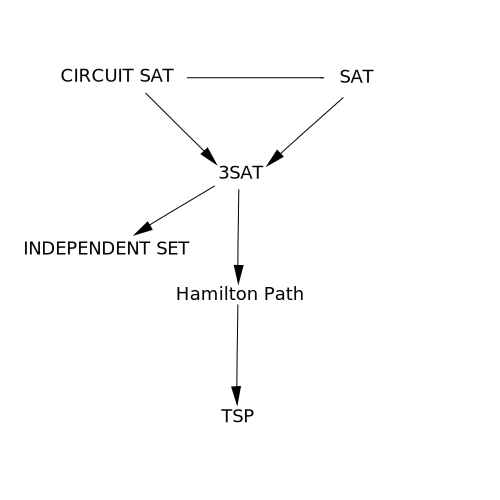
\includegraphics[bb=0 0 400 400,scale=0.5]{./GraphReductionTree.png}
 % GraphReductionTree.png: 1667x1667 pixel, 300dpi, 14.11x14.11 cm, bb=0 0 400 400
\end{center}

Vi vil derfor tage et simpelt eksempel først ved at reducere til en special
case af SAT, kaldet 3SAT.\\

3SAT er en special case af SAT hvor hver klausul skal indeholde præcis 3
literals. Det er et specifikt eksempel på kSAT hvor $k \geq 1$.\\
~\\
\textbf{Proposition 9.2:} 3SAT $\in$ NPC

\begin{proof}
 Vi vil, som sagt, vise at 3SAT $\in$ NPC ved at lave en reduktion fra SAT,
 således vi bruger et polynomial time computable map til at oversætte enhver
 instans af SAT til en instans af 3SAT. 

Givet en CNF formel $f$ i SAT vil vi konstrukere en ny CNF formel $f' = r(x)$ i
3SAT med 3 literals i hver klausul. $r$ er således vores polynomial time
computable map der ændrer følgende i $f$:\\

For hver klausul $k$ i $f$ med literals $x_1, \hdots, x_{|k|}$ ændres:
\begin{itemize}
 \item Hvis $|k| = 2$: Dupliker klausulen og tilføj en ny variabel i begge hvor
	 den negeres i anden klausul \\
      $(x_1 \vee x_2) \rightarrow (x_1 \vee x_2 \vee u) \wedge (x_1 \vee x_2 \vee \neg u)$
 \item Hvis $|k| = 1$: Gør som ved $|k| = 2$, men gør det to gange \\
	  $(x_1) \rightarrow (x_1 \vee u_1) \wedge (x_1 \vee \neg u_1) \rightarrow
	  (x_1 \vee u_1 \vee u_2) \wedge (x_1 \vee u_1 \vee \neg u_2) \wedge (x_1
	  \vee \neg u_1 \vee u_2) \wedge (x_1 \vee \neg u_1 \vee \neg u_2)$
 \item Hvis $|k| = 3$: Gør vi ingenting
 \item Hvis $|k| > 3$: Da vi har en klausul $(x_1,\hdots,x_{|k|})$ så skal vi
	 have en generel måde hvorpå vi kan konvertere dette til klausuler med 3
	 literals. Måden vi gør det på er ved at lave nye variabler
	 $u_1,\hdots,u_{|k|-3}$ og lave en ``kaskade'' af disse:\\
	  $(x_1,\hdots,x_{|k|}) \rightarrow (x_1 \vee x_2 \vee u_1) \wedge (x_3
	  \vee \neg u_1 \vee u_2) \wedge \hdots \wedge (x_{k-2} \vee \neg u_{k-4}
	  \vee u_{k-3}) \wedge (x_{k-1} \vee x_k \vee \neg u_{k-3})$ \\
      ~\\
      Længden af denne udvidelse er så $|k|-2$.
	  For at se at vi kan gøre dette, så skal vi kigge på hvorledes det gamle
	  udtryk har set ud. Hvis det gamle udtryk har været sandt så har et af
	  $x_i$'erne været sat til true. Hvis vi så sætter alle $u_i$'er til true
	  op til punktet hvor $x_i$ blev mødt og falsk derefter, så kan vi se, at
	  det giver et samlet sandt udtryk som før. Det betyder også at hvis ingen
	  $x_i$'er er sat til true og det samlede udtryk derfor burde være falsk,
	  så har vi også bibeholdt dette i oversættelsen, da alle $u_i$'erne derfor
	  må være false.\\
      ~\\
	  \textbf{TODO:} Ovenstående trin for $|k| > 3$ er IKKE rigtig. Jeg har
	  ikke haft tid til at rette det.. Søg på Google og find det rigtige svar.
	  Der findes sider der beskriver beviset.
\end{itemize}

En tilfredsstillende assignment for $f'$ vil altså også være tilfredsstillende
for $f$ og vice-versa. Vi har således lavet en reduktion vha. et polynomial
time computable map $r$, hvor længden af $f'$ maksimalt er $O(|f|^2)$.

Vi har derfor nu vist, at SAT $\leq$ 3SAT, hvorfor vi kan konkludere at 3SAT
$\in$ NPC.
\end{proof}

\subsubsection{Theorem 9.4}

Nu hvor vi så har 3SAT på plads, så kan vi gå videre og kigge på et grafproblem
kaldet INDEPENDENT SET. Vi har en urettet graf $G=(V,E)$. Lad så $I \subseteq
V$, hvor vi kalder $I$ ``independent'' hvis der for alle $i,j \in I$ ikke er en
kant imellem $i$ og $j$. 

INDEPENDENT SET problemet er så: \textit{Givet en urettet graf $G=(V,E)$ og et
mål $K$, er der et independent set $I$ hvor $|I|=K$?}\\
~\\
\textbf{Theorem 9.4:} INDEPENDENT SET $\in$ NPC

\begin{proof}
 For at kunne bevise INDEPENDENT SET er i NPC, så skal vi bruge en lille
 gadget, nemlig en trekant som dem nedenfor. Begrundelsen for dette er, at hvis
 grafen indeholder en trekant, så ved vi på forhånd et independent set
 maksimalt kan indeholde 1 af de 3 knuder i trekanten. Dette bruger vi så i
 beviset ved at vi begrænser den mængde af grafer vi kigger på, til kun at
 tillade grafer vis knuder kan opdeles i $m$ disjunkte trekanter. Således får
 vi at vi maksimalt kan have et independent set af størrelse $m$ (en fra hver
 trekant) og at denne eksisterer hvis og kun hvis kanterne i konstruktionen
 tillader vi kan vælge en knude fra hver trekant.
 \begin{center}
 \includegraphics[bb=0 0 842 595,scale=0.5]{./INDEPENDENTSET.png}
 % INDEPENDENTSET.png: 3508x2480 pixel, 300dpi, 29.70x21.00 cm, bb=0 0 842 595
\end{center}
Konstruktionen i reduktionen fra en 3SAT instans til INDEPENDENT SET kommer så
nemt heraf (illustreret ovenfor). Konstruktionen er som følger:

\begin{enumerate}
 \item For hver af de $m$ klausuler af en given CNF formel $f$ skabes en ny
	 trekant i $G$.
 \item Hver knude i trekanten svarer så til en literal i den pågældende klausul.
 \item Tilføj kanter mellem nodes med modsatte literals (således $x_1$ får en
	 kant til $\neg x_1$).
 \item Sæt målet $K$ i INDEPENDENT SET problemet til $m$.
\end{enumerate}

Herefter er konstruktionen færdig. Vi påstår så nu, at der er et independent
set af $K$ nodes i $G$ hvis og kun hvis $f$ tilfredsstilles. Hvis vi antager
sådan et independent set $I$ eksisterer, så siden $K=m$, så må $I$ indeholde en
knude pr. trekant. Siden alle nodes er labeled med deres literal og $I$ ikke
indeholder to knuder svarende til modsatte literals, så er $I$ en sandt/falsk
tildeling der tilfredsstiller $f$. Alle literals indeholdt i $I$ bliver så dem
der er ``true''.

Og set fra den anden side, så hvis vi ved $f$ har en tilfredstillende
tildeling, så identificerer vi blot de literals der bliver ``true'' i $f$ og
markerer dem som en del af $I$ i grafen $G$, hvorved vi får et independent set
med $m=K$ uafhængige knuder.

Vi har derved bevist at 3SAT $\leq$ INDEPENDENT SET, hvorved vi kan konkludere
INDEPENDENT SET $\in$ NPC.
\end{proof}

\subsubsection{Theorem 9.7}

Nu har vi så gået i en retning med reduktioner fra 3SAT og vil nu gå i en ny
retning, nemlig mod problemet HAMILTON PATH. 
HAMILTON PATH problemet er så: \textit{Givet en urettet graf $G=(V,E)$, har $G$
en Hamilton path, altså en sti der besøger hver knude præcis en gang?}\\
~\\
\textbf{Theorem 9.7:} HAMILTON PATH $\in$ NPC

\begin{proof}
 Det vi ønsker at bevise er, at HAMILTON PATH er NP-Complete og måden vi gør
 det på er ved at reducerer fra 3SAT. Så vi skal vise at 3SAT $\leq$ HAMILTON
 PATH.

Så fra 3SAT har vi altså en CNF formel $f$ med variabler $x_1,\hdots,x_n$ og
klausuler $C_1,\hdots,C_m$, hver med 3 literals. Vi konstruerer så en graf $G =
r(f)$ med en Hamilton Path hvis og kun hvis formel $f$ tilfredsstilles.
Vi skal altså finde en måde at modellere 3SAT vha. HAMILTON PATH, således vi
har ækvivalenten af nogle boolske variabler, muligheden for at sætte dem til
sandt/falsk, en ækvivalent af klausuler som constraints, samt muligheden for at
bibeholde konsistens således $x_i$ altid har samme værdi og $\neg x_i$ altid
har den modsatte værdi heraf.\\

I vores tilfælde gør vi dette vha. nogle gadgets. Den første af disse er en
såkaldt ``choice gadget'', som illustreret herunder.
\begin{center}
 \includegraphics[bb=0 0 499 842,scale=0.2]{./choiceGadget.png}
 % choiceGadget.png: 2080x3508 pixel, 300dpi, 17.61x29.70 cm, bb=0 0 499 842
\end{center}
Denne gadget skal så bruges som en delgraf forbundet til resten vha. de sorte
knuder. Vores choice gadget vil så gøre, at vi kan tildele forskellige
sandhedsværdier afhængig af hvilken kant Hamilton stien vælger ned igennem
delgrafen og derved modellere en boolsk variabel. 

Så nu har vi boolske variabler på plads, nu mangler vi en gadget til at
håndtere consistency. Måden hvorpå vi gør dette er vha. følgende ``consistency
gadget''.

\begin{center}
 \includegraphics[bb=0 0 173 81]{./consistencyGadget.png}
 % consistencyGadget.: 231x108 pixel, 96dpi, 6.11x2.86 cm, bb=0 0 173 81
\end{center}

Hvis denne gadget kobles til en omkringliggende graf vha. de sorte knuder, så
kan vi se at en given Hamilton Path kun har 2 mulige veje at gå igennem grafen.
Uanset hvad er den nød til at zig-zag op og ned langs grafen for at kunne
besøge alle knuder, så det eneste der kan varieres er hvilken sort knude den
starter udfra. Vi får altså egenskaben, at denne gadget nærmest opfører sig som
to separate kanter hvor en kant besøges af Hamilton stien og den anden gør
ikke. Vi kan altså tænke på denne gadget som en form for XOR mellem to kanter:

\begin{center}
 \includegraphics[bb=0 0 173 81]{./consistencyGadget2.png}
 % consistencyGadget.: 231x108 pixel, 96dpi, 6.11x2.86 cm, bb=0 0 173 81
\end{center}

Så nu har vi en consistency gadget på plads, så mangler vi bare at håndtere
klausuler. Men til dette kan vi heldigvis bruge en gammel kending, nemlig
trekanten. Modsat brugen i INDEPENDENT SET, så vælger vi dog her at tildele en
literal til hver kant. Ved at gøre dette, så kan vi sige en given literal er
``false'' såfremt den indgår i den pågældende Hamilton Path. Derved har vi
også, at minimum en literal er nød til at være ``true'', da der ellers ikke er
nogen Hamilton Path. Vores ``constraint gadget'' ser så således ud:

\begin{center}
 \includegraphics[bb=0 0 241 185]{./constraintGadget.png}
 % constraintGadget.png: 322x247 pixel, 96dpi, 8.52x6.53 cm, bb=0 0 241 185
\end{center}

Hvis vi så sætter alle de her ting sammen så får vi følgende opskrift:\\
\begin{enumerate}
 \item Konstruer en graf $G$ med en start knude kaldet 1.

 \item Lav $n$ kopier af vores ``choice gadget'', en for hver variabel, og
	 forbind dem i en serie efter 1.

 \item Lav $m$ trekanter, en for hver klausul, og forbind dem således kanten
	 der svarer til $x_i$ er forbundet vha. vores ``consistency gadget'' til
	 kanten i vores ``choice gadgets'' der svarer til true-kanten for variablen
	 $x_i$, således trekantens kant traverseres hvis ``choice gadget`` kanten
	 ikke gør. Og tilsvarende hvis en kant svarer til $\neg x_i$ så forbind den
	 vha. en ``consistency gadget'' til false-kanten på den tilsvarende
	 variables ``choice gadget''. 
	 \textit{OBS: der kan godt være flere ``consistency gadgets'' der går til
	 samme kant i en ``choice gadget'', men ikke den anden vej rundt.}

 \item Herefter skabes en clique indeholdende de $3m$ trekant knuder, den
	 sidste knude i serien af ``choice gadgets'', samt en ny knude kaldet 3.
	 \textit{OBS: En clique er bare et sæt af knuder hvor alle mulige kanter
	 eksisterer imellem dem}

 \item Slutteligt tilføjes en enkelt knude kaldet 2 og forbindes til 3.

\end{enumerate}
Herefter har vi konstrueret vores graf, som er illustereret nedenfor:

\begin{center}
 \includegraphics[bb=0 0 350 440]{./hamiltonPath.png}
 % hamiltonPath.png: 467x587 pixel, 96dpi, 12.35x15.53 cm, bb=0 0 350 440
\end{center}

Vi påstår så nu, at grafen har en Hamilton Path hvis og kun hvis $f$ har en
tilfredsstillende tildeling. Lad os antage en sådan Hamilton Path eksisterer,
så må start og slut på stien være henholdsvis knude 1 og knude 2. Hvis vi så
starter fra knude 1, så må stien gå ned igennem de pågældende ``choice
gadgets'' ved enten at tage kanten der svarer til ``true`` eller kanten der
svarer til ''false``. Desuden skal alle XORs traverseres, således vi i sidste
ende får at hele kæden af valg bliver traverseret. Hele denne sti definerer så
en tildeling af sandhedsværdier, som vi kalder $T$. Efter dette traverseres
trekanterne i en eller anden rækkefølge hvorefter vi ender ved knude 2.\\

Vi påstår så $T$ tilfredsstiller $f$, da alle XORs bliver traverseret på en
måde hvor de fungerer som XOR, da en trekants side svarende til en literal, kun
traverseres hvis den literal var ''false``. Derved siden der ingen klausuler er
for hvilket alle literals er ''false``, så er $f$ tilfredsstillet.

Og set fra den anden side hvor vi har en given tildeling $T$ der
tilfredsstiller $f$, så kan vi bruge $r(f)$ til at skabe en graf med en
Hamilton Path der starter fra knude 1. Herefter traverserer den ned igennem
valgmulighederne og følger kanterne svarende til værdierne i $T$. Efter dette
er gjort er resten af grafen en stor clique, som så bliver traverseret indtil
stien slutter ved knude 2.

Vi har således vist at 3SAT $\leq$ HAMILTON PATH, og derved at HAMILTON PATH
$\in$ NPC.
\end{proof}


\subsubsection{Collary: (TSP $\in$ NPC)}

Nu hvor vi har HAMILTON PATH på plads som NPC, så kan vi også slutteligt lige
argumentere for at TSP ligeledes er det, ved at lave et  simpelt bevis.\\

\textbf{Collary: $TSP(D) \in NPC$}

\begin{proof}
 Vi vil vise TSP er NP-Complete ved at reducere fra HAMILTON PATH. Dette gør vi
 ved at vi har en graf $G=(V,E)$ i HAMILTON PATH, og vi vil så konstruere en ny
 graf i TSP således $G' = r(G)$. Hertil skal vi også opbygge en distance matrix
 $d_{ij}$ således følgende gælder:

\begin{itemize}
 \item Hvis $[i,j]$ er en kant i $G$, så sæt $d_{ij}=1$.
 \item Ellers sæt $d_{ij}=2$.
\end{itemize}

Vi skal også have et budget $B$ således at der er en rute af længde $B$ eller
mindre hvis og kun hvis $G$ har en Hamilton Path. Der er desuden $n$ byer, en
for hver knude i grafen $G$. Sidst men ikke mindst sættes $B=n+1$.
Konstruktionen er herefter fuldendt.\\

Vi påstår så nu, at $G'$ har en rute med distance højst $B$ hvis og kun hvis
$G$ har en Hamilton Path. Hvis vi først antager, at $G$ har en Hamilton Path,
så vil der være en rute i $G'$ for hvilken den samlede distance er mindre end
$B$ da $B=n+1$ og der kun er $n$ byer. Hvorimod hvis vi antager der ikke er en
Hamilton Path, så vil der heller ikke være en rute i $G'$ da en given rute vil
have distance på $2(n-1) > B$.

Vi har derved vist at ovenstående er en korrekt reducering af HAMILTON PATH til
TSP, så HAMILTON PATH $\leq$ TSP, og derved gælder der at TSP $\in$ NPC.
\end{proof}


\section{NP-complete problems involving sets and numbers.}

\subsection{Disposition}

\begin{enumerate}
 \item \textbf{Def. P, NP, NP-hard \& NPC}
    \subitem  Tegn!
 \item \textbf{Def. Reduktioner}
    \subitem  Proposition 3: Transitivitet (v. bevis)
    \subitem  Proposition 4: Nedadgående lukkethed af P  
 \item \textbf{Lemma 7:} \textit{Hvis $L_1 \in$ NP-hard og $L_1 \leq L_2$, så er $L_2 \in$ NP-hard}
    \subitem  Bevis. (måske)
 \item \textbf{Reduktionstræ}
 \item \textbf{Proposition 9.2:} \textit{3SAT $\in$ NPC}
    \subitem Vis SAT $\leq$ 3SAT. (måske)
 \item \textbf{Theorem 9.9:} \textit{3SAT $\leq$ TRIPARTITE MATCHING}
    \subitem Bevis
 \item \textbf{Collary:} \textit{EXACT COVER BY 3-SETS, SET COVERING and SET PACKING are NPC}
    \subitem Vis for EXACT COVER BY 3-SETS
 \item \textbf{Theorem:} \textit{EXACT COVER BY 3-SETS $\leq$ KNAPSACK}
    \subitem Bevis
\end{enumerate}

\subsection{Emne detaljer}

Følgende afsnit indeholder detaljer om hvert punkt i dispositionen ovenfor (og muligvis flere ting også).

\subsubsection{Def. P, NP, NP-hard \& NPC}

Lad os starte med lige at kigge på de kompleksitetsklasser vi har arbejdet med her i kurset.
\begin{center}
 \includegraphics[bb=0 0 400 400,scale=0.3]{img/PNPNPC.png}
 % PNPNPC.png: 1667x1667 pixel, 300dpi, 14.11x14.11 cm, bb=0 0 400 400
\end{center}


\paragraph{P}
~\\
~\\
Kompleksitetsklassen $P$ er formelt defineret således:
\begin{align*}
 P = \left\lbrace L \subseteq \left\lbrace 0,1 \right\rbrace^* | \exists \text{ TM } M_L \text{ der afgører L i polynomiel tid } \right\rbrace
\end{align*}
Altså klassen af beslutningsproblemer der kan blive bestemt af en deterministisk Turing Maskine hvor antallet af ``steps'' maskinen udfører for et givent $x$ maksimalt er $\rho(x)$ for et givent polynomiel $\rho$.\\
 
Intuivit ser vi kompleksitetsklassen $P$ som en klasse for problemer for hvilket vi kender en effektiv løsning. Altså ethvert problem med worst-case kørselstid på formen $O(n^k)$ for et givent $k$.

At worst-case kørseltid på et problem er polynomiel betyder dog ikke reelt at det er et nemt problem (modsat hvad Cobham's Thesis påstår). I hele den analyse ignorerer vi fuldkommen konstanter, samt forventet kørselstid som I mange tilfælde kan få ``sværere'' problemer til at køre bedre end ``nemme'' problemer i $P$.


\paragraph{NP}
~\\
~\\
Kompleksitetsklassen $NP$ er lidt mere kluntet formelt defineret, så vi starter lige med intuitionen først.

Intuitivt kan $NP$ ses som klassen af beslutningsproblemer for hvilket ``yes'' instanserne kan verificeres i polynomiel tid på en deterministisk Turing Maskine. Altså er det komplekse problemer med eksponentiel løbetid, men hvor løsningen til et sådant problem nemt kan verificeres til at være korrekt.\\
~\\
Kompleksitetsklassen $NP$ er formelt defineret således:
\begin{align*}
 NP = \left\lbrace L \subseteq \left\lbrace 0,1 \right\rbrace^* | \exists \rho \in Z[x], L' \in P, \forall x \in \left\lbrace 0,1 \right\rbrace^* : ( x \in L \Leftrightarrow \exists y \in \left\lbrace 0,1 \right\rbrace^* : |y| \leq \rho(|x|) \wedge \left\langle x,y \right\rangle \in L') \right\rbrace
\end{align*}
Definitionen skal forståes således: Vi har et sprog $L' \in P$, samt et polynomiel $\rho$. Vi tænker så nu på et sæt af binære strenge af længde maksimalt $\rho(|x|)$, hvor disse representerer mulige løsninger til probleminstansen $x$. Med denne fortolkning bliver $\left\langle x,y \right\rangle \in L'$ så måden hvorpå vi tester om en given løsning $y$ virkelig er en korrekt løsning. 

Denne form for søgningsproblem kaldes ofte for et simpelt søgningsproblem, da den kan verificeres i polynomiel tid, men ikke løses deri (antaget $P \neq NP$).\\

For at løse et givent NP problem kunne vi så løbe igennem alle mulige løsninger for $y$, som sammenlagt ville være $2^{\rho(|x|)+1}-1$, og for hver af dem tjekke $\left\langle x,y \right\rangle \in L'$. Det ønsker vi dog ikke, da det ville tage eksponentiel tid. I stedet forsøger man ofte at finde snedige måder at lave speed-ups og/eller lave approximationsalgoritmer af forskellige art.

Og i visse tilfælde er man også heldig at finde en algoritme i $P$ for et $NP$ problem, hvorved man har vist at problemet i virkeligheden ligger i $P$ som jo er et subset af $NP$.

\paragraph{NP-hard}
~\\
~\\
Et sprog defineres som NP-hard såfremt der gælder:

\begin{align*}
 \forall L' \in NP: L' \leq L
\end{align*}

Altså gælder der, at ethvert sprog $L'$ i NP kan reduceres til $L$. Intuitionen er her, at algoritmen til at løse NP-hard problemet er så stærk (eller generel) at den kan bruges til at løse ethvert andet problem i NP. Man siger desuden, at et NP-hard problem således er mindre sandsynlig end noget andet sprog i NP, til at være i P.\\

Navnet kan dog være lidt forvirrende, da et NP-hard problem faktisk ikke behøver være i NP og hvis de er, så kaldes de faktisk ikke engang bare NP-hard længere.

\paragraph{NPC}
~\\
~\\
NP-Complete (NPC) er den særlige klasse af problemer der både er NP-hard og befinder sig i NP. Formelt defineret således: 

\begin{align*}
 NPC = \left\lbrace L \in \left\lbrace 0,1 \right\rbrace^* | L \in NP \wedge (\forall L' \in NP: L' \leq L) \right\rbrace
\end{align*}

NPC problemer er særligt interessante, da vi kan bruge dem til at bevise et givent problem er NP-Complete, således vi ikke spilder tid på forsøg med at finde en algoritme i $P$ for problemet (antaget $P\neq NP$). Dette gør vi vha. noget vi kalder reduktioner.

\subsubsection{Def. Reduktioner}

Det bringer os så til en grundlæggende metode i computationel kompleksitetsteori, nemlig reduktioner. Først og fremmest den formelle definition.

Givet to sprog $L_1$ og $L_2$, en polynomiel reduktion $r$ af $L_1$ til $L_2$ er en polynomial time computable map for hvilken der gælder:

\begin{align*}
 \forall x : x \in L_1 \text{ hviss. } r(x) \in L_2
\end{align*}

Dette skrives som $L_1 \leq L_2$, hvor man læser det som at $L_1$ reduceres til $L_2$. Intuitivt betyder reduktion blot, at vi kan oversætte enhver given instans af $L_1$ til en anden instans af $L_2$. Vi siger desuden, at $L_2$ er et mere generelt sprog end $L_1$ og kan derfor ses, som værende mere sandsynlig til ikke at være i $P$.


Herudover har  reduktioner desuden to nyttige egenskaber vi skal bruge senere.

\paragraph{Proposition 3: Hvis $L_1 \leq L_2$ og $L_2 \leq L_3$, så gælder der $L_1 \leq L_3$}
~\\
~\\
Denne proposition underbygger, at reduktioner er transitive. Vi beviser den således:

\begin{proof}
 Vi har polynomial time computable maps $r_1()$ og $r_2()$, hvor følgende ting gælder:

\begin{itemize}
 \item For ethvert $x$ gælder der, at $x \in L_1$ hvis og kun hvis $r_1(x) \in L_2$.
 \item For ethvert $y$ gælder der, at $y \in L_2$ hvis og kun hvis $r_2(y) \in L_3$.
\end{itemize}

Således har vi for alle $x$, at $x \in L_1$ hvis og kun hvis $r_2(r_1(x)) \in L_3$. Og siden vi blot har brugt to polynomial time computable maps efter hinanden (hvormed det hele kan ses som en polynomial time computable map), så har vi $L_1 \leq L_3$.
\end{proof}

\paragraph{Proposition 4: Hvis $L_1 \leq L_2$ og $L_2 \in P$, så er $L_1 \in P$.}

Proposition 4 siger intuitivt, at $P$ er lukket nedad under reduktion. 


\subsubsection{Cook's Theorem}

Vi vil jo gerne kunne vise at diverse problemer er NP-Complete, men for at gøre det vha. reduktioner, så skal vi først have et NP-Complete problem at starte ud fra.

Takket være Stephen Cook fik vi i 1972 netop lige det, da han viste at SATISFIABILITY PROBLEMET, forkortet SAT, var NP-hard. Herefter kunne mange andre så bruge SAT til at reducere til andre problemer, for at vise at disse nye problemer var NP-hard. Cook beviste oprindeligt SAT ved at vise alle problemer i NP reducerede til SAT, hvilket er en noget kompliceret affære. Derfor har vi i dette kursus i stedet vist et relateret problem CIRCUIT SAT er NP-hard og så reduceret dette til SAT.

Det vil vi dog ikke gøre til dette emne og vil i stedet blot definere problemerne samt deres kompleksitet, så vi kan bruge dem til at lave andre reduktioner.

\begin{itemize}
 \item CIRCUIT SAT $\in$ NPC (Theorem 11)
 \item CIRCUIT SAT $\leq$ SAT (Proposition 12)
\end{itemize}

\paragraph{Def. SAT}
~\\
~\\
Givet en CNF formel, er der en tildeling af sandt/falsk til variablerne således hele udtrykket evaluerer til sandt?\\

\paragraph{Def. CIRCUIT SAT}
~\\
~\\
Givet et boolsk kredsløb $C$, er der en inputvektor $x \in \left\lbrace 0,1 \right\rbrace^n$ således at $C(x) = 1$?

\subsubsection{Proposition 9.2}

Vi ved som sagt, at SAT er et NP-Complete problem, så kan vi bruge det til at bevise andre problemer er NP-Complete ved at reducere SAT til dem.
Specifikt er det planen at gennemgå følgende reduktioner i løbet af dette emne:
\begin{center}
 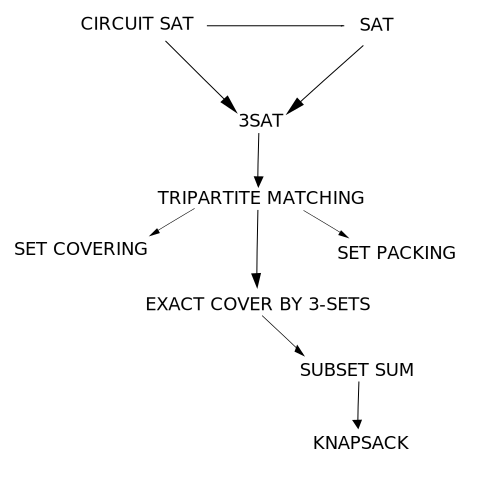
\includegraphics[bb=0 0 400 400,scale=0.5]{img/GraphReductionTreeSetNumbers.png}
 % GraphReductionTree.png: 1667x1667 pixel, 300dpi, 14.11x14.11 cm, bb=0 0 400 400
\end{center}

Vi vil derfor tage et simpelt eksempel først ved at reducere til en special case af SAT, kaldet 3SAT.\\
3SAT er en special case af SAT hvor hver klausul skal indeholde præcis 3 literals. Det er et specifikt eksempel på kSAT hvor $k \geq 1$.\\
~\\
\textbf{Proposition 9.2:} 3SAT $\in$ NPC

\emph{Bevis.} Vi vil, som sagt, vise at 3SAT $\in$ NPC ved at lave en reduktion fra SAT, således vi bruger et polynomial time computable map til at oversætte enhver instans af SAT til en instans af 3SAT. 

Givet en CNF formel $f$ i SAT vil vi konstrukere en ny CNF formel $f' = r(x)$ i 3SAT med 3 literals i hver klausul. $r$ er således vores polynomial time computable map der ændrer følgende i $f$:\\

For hver klausul $k$ i $f$ med literals $x_1, \hdots, x_{|k|}$ ændres:
\begin{itemize}
\item Hvis $|k| = 2$: Dupliker klausulen og tilføj en ny variabel i
begge hvor den negeres i anden klausul \\ $(x_1 \vee x_2) \rightarrow
(x_1 \vee x_2 \vee u) \wedge (x_1 \vee x_2 \vee \neg u)$
\item Hvis $|k| = 1$: Gør som ved $|k| = 2$, men gør det to gange \\
  $(x_1) \rightarrow (x_1 \vee u_1) \wedge (x_1 \vee \neg u_1)
  \rightarrow (x_1 \vee u_1 \vee u_2) \wedge (x_1 \vee u_1 \vee \neg
  u_2) \wedge (x_1 \vee \neg u_1 \vee u_2) \wedge (x_1 \vee \neg u_1
  \vee \neg u_2)$
\item Hvis $|k| = 3$: Gør vi ingenting
\item Hvis $|k| > 3$: Da vi har en klausul $(x_1,\hdots,x_{|k|})$ så
  skal vi have en generel måde hvorpå vi kan konvertere dette til
  klausuler med 3 literals. Måden vi gør det på er ved at lave nye
  variabler $u_1,\hdots,u_{|k|-3}$ og lave en ``kaskade'' af disse:\\
  $(x_1,\hdots,x_{|k|}) \rightarrow (x_1 \vee x_2 \vee u_1) \wedge
  (\neg u_1 \vee x_3 \vee u_2) \wedge (\neg u_2 \vee x_4 \vee u_3 )
  \wedge
  \hdots \wedge (\neg u_{k-3} \vee x_{k-1} \vee x_{k} ) $ \\
  ~\\
  Længden af denne udvidelse er så $|k|-2$.  For at se at vi kan gøre
  dette, så skal vi kigge på hvorledes det gamle udtryk har set
  ud. Hvis det gamle udtryk har været sandt så har et af $x_i$'erne
  været sat til true. Hvis vi så sætter alle $u_i$'er til true op til
  punktet hvor $x_i$ blev mødt og falsk derefter, så kan vi se, at det
  giver et samlet sandt udtryk som før. Det betyder også at hvis ingen
  $x_i$'er er sat til true og det samlede udtryk derfor burde være
  falsk, så har vi også bibeholdt dette i oversættelsen, da
  alle $u_i$'erne derfor må være false.\\
  ~\\
\end{itemize} 

En tilfredsstillende assignment for $f'$ vil altså også være
tilfredsstillende for $f$ og vice-versa. Vi har således lavet en
reduktion vha. et polynomial time computable map $r$, hvor længden af
$f'$ maksimalt er $O(|f|^2)$.

Vi har derfor nu vist, at SAT $\leq$ 3SAT, hvorfor vi kan konkludere
at 3SAT $\in$ NPC.

\subsubsection{Theorem 9.9}

\textbf{TODO: } Følgende bevis har jeg ikke ordentligt forstået og kan meget vel være forkert hernede.. Tjek den efter meget grundigt og få ekstra kilder hvorfra du kan verificere nedenstående.. Beviset fuldføres heller ikke helt, som kan ses nedenfor. \\
~\\
Nu hvor vi har fastlagt at 3SAT er i NPC, så kan vi bruge den til at reducere videre. Så det første vi vil kigge på er et beslutningsproblem relateret til set, kaldet TRIPARTITE MATCHING (oversat: treparts matching)

TRIPARTITE MATCHING problemet er følgende: Vi er givet tre sæt $B$, $G$ og $H$ respektivt indeholdende drenge, piger og hjem. Hvor hver af disse sæt indeholder $n$ elementer og vi har en relation $T \subseteq B \times G \times H$. Findes der nu et sæt af $n$ tripler i $T$, hvor ingen to af disse har komponenter til fælles. \\

Altså sagt på en anden måde, kan vi finde $n$ tripler hvor hver dreng er koblet med en pige og disse så er placeret i et hjem.

Dette problem er NP-Complete, hvilket vi så nu vil vise.
\\
~\\
\textbf{Theorem 9.9:} TRIPARTITE MATCHING $\in$ NPC

\begin{proof}
 Vi vil vise at TRIPARTITE MATCHING er i NPC ved at reducerer fra 3SAT. Vi har altså en CNF formel $f$ i 3SAT med variabler $x_1,\hdots,x_n$ og skal så nu konstruere instanser af TRIPARTITE MATCHING på baggrund af dette vha. en polynomieltids reduktion $r$.

 Måden hvorpå vi konstruerer disse instanser er vha. en såkaldt ``choice-consistency'' gadget, som illustreret nedenfor.
 \begin{center}
 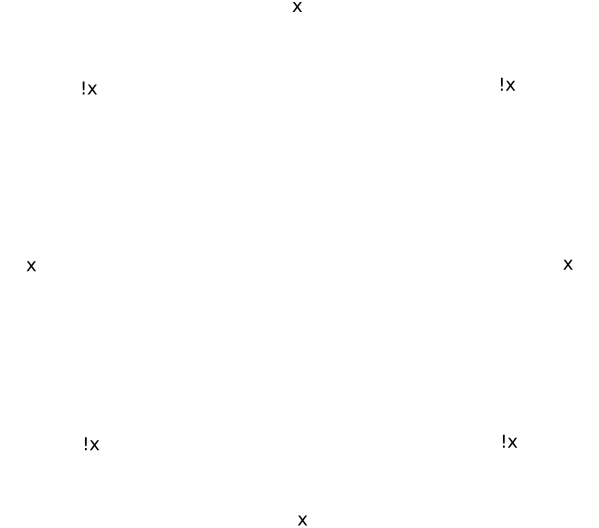
\includegraphics[bb=0 0 479 422,scale=0.5]{img/choiceConsistency.png}
 % choiceConsistency.png: 1997x1760 pixel, 300dpi, 16.91x14.90 cm, bb=0 0 479 422
\end{center}
Konstruktionen følger så denne opskrift:
\begin{enumerate}
 \item For hver variabel $x_i$ i $f$, konstruer en ``choice-consistency'' gadget
    \subitem (a) Lad $k$ være antallet af forekomster af $x_i$, eller $\neg x_i$, i $f$ (den af dem hvor der er flest).
    \subitem (b) Konstruer vores gadget med $k$ drenge, $k$ piger og $2k$ hjem. Hvor drenge og piger placeres efter hinanden i en slags ``ring'' hvor hjemene er placeret ud for dem i en trekant repræsenterende tripler.
    \subitem (c) Hjemene $h_{2i-1}$ repræsenterer forekomster af $x$, hvor $h_{2i}$ repræsenterer forekomster af $\neg x$, for $i = 1,\hdots,k$. (hvis antallet af forekomster af de to er ulige, så vil nogle $h_i$'er blot være utildelt)
    \subitem (d) De $k$ drenge og $k$ piger indgår ikke i tripler af $T$ udover dem der er vist i figuren. Så hvis en matching eksisterer, så er $b_i$ matched med $g_i$ og $h_{2i}$ eller med $g_{i-1}$ ($g_k$ hvis $i=1$) og $h_{2i-1}$, for $i = 1,\hdots,k$. Hvis den første var tilfældet, så er $T(x)=true$ og hvis det er den anden så er $T(x)=false$. \\
    Dette betyder, at en given variabel $x$ altid vælger en tildeling og alle forekomster af variablen har konsistente værdier.
 \item For hver klausul i $f$, konstruer en triple med en dreng $b$ og en pige $g$. De eneste tripler $b$ og $g$ indgår i, er så tripler på formen $(b,g,h)$ hvor $h$ er de 3 hjem svarende til de 3 forekomster af literals i den pågældende klausul. Ideen er så, at hvis en af disse 3 hjem blev efterladt ubeboet når variabler blev tildelt værdier, så betyder det at huset svarer til en ``true'' literal og klausulen er derfor tilfredsstillet. Hvis alle 3 literals i klausulen er ``false'', så kan $b$ og $g$ ikke tildeles et hjem. \\
 Illustreret nedenfor:
\end{enumerate}
\begin{center}
 \includegraphics[bb=0 0 292 174]{img/choiceConsistencySub.png}
 % choiceConsistencySub.png: 389x232 pixel, 96dpi, 10.29x6.14 cm, bb=0 0 292 174
\end{center}


Hermed er konstruktionen færdig, dog med den detalje at der pt. er flere hjem end drenge og piger i konstruktionen. Hvis der er $m$ klausuler, så er der $3m$ forekomster hvorfor der mindst er $H=3m$ hjem (for hver variabel har vi mindst lige så mange hjem som forekomster). På den anden side har vi $\frac{H}{2}$ drenge i vores gadgets og yderligere $m \leq \frac{H}{3}$ i vores klausul constraint del.

Lad os antage at mængden af huse vi har for meget er $l$, så kan vi introducere $l$ flere drenge og $l$ flere piger, således $|B| = |G| = |H|$. For hver af disse $l$ drenge og piger tilføjes så $|H|$ tripler der forbinder til alle hjem. Disse sidste $l$ drenge og piger kan så ses som ``easy to please'' par, da de blot bruges til at udfylde hvad end hjem der er ubeboet.\\
~\\
Vi påstår så nu, at en tripartite matching eksisterer hvis og kun hvis den oprindelige boolske formel var tilfredsstillet. Dette kan vi se ved 
 
\end{proof}



\subsubsection{Collary: Andre problemer med sæt i NPC}

Nu hvor vi har bevist at TRIPARTITE MATCHING er NP-Complete, så bringer det nærmest automatisk en række andre problemer ind i den kategori, da visse andre problemer med sæt blot er forskellige afarter heraf. Her kigger vi specifikt på 3 hurtigt, nemlig EXACT COVER BY 3-SETS, SET COVERING og SET PACKING. Problemerne er defineret således:

\begin{description}
 \item[SET COVERING:] Vi er givet en familie $F = \left\lbrace S_1,\hdots,S_n \right\rbrace$ af subsets af et endeligt sæt $U$ og et budget $B$. Er der et sæt af $B$ sæt i $F$ hvor deres foreningsmængde er $U$?
 \item[SET PACKING:] Vi er givet en familie $F = \left\lbrace S_1,\hdots,S_n \right\rbrace$ af subsets af et sæt $U$ og et mål $K$. Er der $K$ parvis disjunkte sæt i familien $F$?
 \item[EXACT COVER BY 3-SETS:] Vi er givet en familie $F = \left\lbrace S_1,\hdots,S_n \right\rbrace$ af subsets af et sæt $U$, således at $|U|=3m$ for en given int $m$ og $|S_i|=3$ for alle $i$. Er der $m$ sæt i $F$ som er disjunkte og har $U$ som deres foreningsmængde?
\end{description}

Alle disse problemer kan vises at være NP-Complete, da de alle er generaliseringer af TRIPARTITE MATCHING.\\
~\\
\textbf{Collary:} EXACT COVER BY 3-SETS, SET COVERING og SET PACKING $\in$ NPC

\begin{proof}
 Vi starter med at reducere TRIPARTITE MATCHING til EXACT COVER BY 3-SETS, for derved at vise, at sidstnævnte er i NPC.

 Givet sæt $B$, $G$ og $H$, samt relationen $T \subseteq B \times G \times H$ i TRIPARTITE MATCHING, så vil vi konstruere disse dele i EXACT COVER BY 3-SETS vha. en polynomiel reduktion $r$. Således kan vi sige, at EXACT COVER BY 3-SETS har $m$ sæt der er disjunkte og har foreningsmængde $U$, hvis og kun hvis TRIPARTITE MATCHING har en fyldestgørende matching.

 Måden vi gør det på er ved at dele $U$ i sidstnævnte op, således $U = B \bigcup G \bigcup H$ hvor disse $B$, $G$ og $H$ selvfølgelig er disjunkte. Til enhver triple $t_i=(b,g,h) \in T$ associerer vi så et sæt $S_i=\left\lbrace b,g,h \right\rbrace$
 Således får vi, at foreningsmængden af de $m$ sæt kun er $U$ såfremt $T$ er en fyldestgørende matching, og vice-versa.
 
 Altså har vi at EXACT COVER BY 3-SETS $\in$ NPC.\\
~\\
Et endnu nemmere bevis kan føres for SET COVERING ved at reducere fra EXACT COVER BY 3-SETS. Vi lader blot $F$ udelukkende bestå af sæts med 3 elementer, lader $U$ bestå af $3m$ elementer og sætter budgettet $B=m$, derved får vi EXACT COVER BY 3-SETS direkte. 

Så SET COVERING $\in$ NPC.\\
~\\
Det tilsvarende kan gøres igen for en reducering fra EXACT COVER BY 3-SETS til SET PACKING, hvor $F$ og $U$ sættes som før, og målet $K=m$. 

Således får vi også her at SET PACKING $\in$ NPC.
\end{proof}

\subsubsection{Theorem: (EXACT COVER BY 3-SETS $\leq$ KNAPSACK)}

Nu hvor vi har vist at EXACT COVER BY 3-SETS er NP-Complete, så kan vi nu bruge den viden til at lave endnu en reduktion. Vi vil kigge på problemet kaldet KNAPSACK.

Problemet går ud på at vi må vælge nogle genstande blandt $n$ samlede genstande. Genstand $i$ har værdi $v_i$ og vægt $w_i$, hvor begge er positive heltal. Der er desuden en max vægt på $W$, som er den maksimale vægt vores genstande tilsammen må veje. Vi skal så nu vælge genstande, uden gentagelser, således vi maksimerer den totale værdi med den constraint at den samlede vægt ikke må overstige $W$.

Vi leder altså efter et subset $S \subseteq \left\lbrace 1,\hdots,n \right\rbrace$ således at $\sum_{i \in S} w_i \leq W$ og $\sum_{i \in S} v_i$ er så stor som mulig.

I beslutningsproblem varianten har vi desuden et mål $K$ og vi ønsker at finde et subset $S \subseteq \left\lbrace 1, \hdots, n \right\rbrace$ således $\sum_{i \in S} w_i \leq W$ og $\sum_{i \in S} v_i \geq K$.

Vi vil så nu bevise at KNAPSACK $\in$ NPC ved at bevise et relateret problem.\\
~\\
\textbf{Theorem 9.10:} KNAPSACK $\in$ NPC

\begin{proof}
 I dette bevis vil vi reducere fra EXACT COVER BY 3-SETS, men vi vil ikke reducere til KNAPSACK. I stedet vil vi begrænse problemet og fokusere på et special case, som vi så vil bevise er NPC. Dette special case kalder vi SUBSET SUM og det eneste vi ændrer imellem de to, er at $K=W$ og for hver genstand $i$ sætter vi $v_i = w_i$.

Altså har vi nu et problem hvor vi er givet et sæt af $n$ heltal $v_1,\hdots,v_n$ og endnu et heltal $K$. Vi ønsker nu at finde ud af om et givet subset summer præcist op til $K$.\\

 Vi har altså en instance af EXACT COVER BY 3-SETS med sæt $\left\lbrace S_1, S_2,\hdots,S_n \right\rbrace$, hvor vi spørger om der er disjunkte sæt hvor deres foreningsmængde er sættet $U = \left\lbrace 1, 2, \hdots, 3m \right\rbrace$. Vi tænker på disse sæt som bit vektorer i $\left\lbrace 0,1 \right\rbrace^{3m}$, således de også kan tænkes som binære heltal og forening mellem disse sæt nu ligner heltalsaddition til forveksling (eksempel ses nedenfor)
\begin{center}
 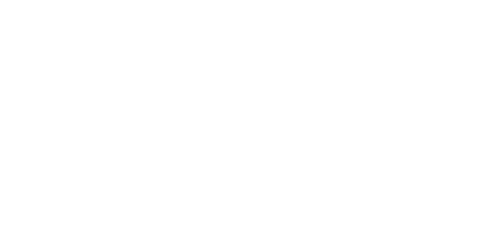
\includegraphics[bb=0 0 389 186,scale=0.5]{img/KNAPSACK.png}
 % KNAPSACK.png: 1620x773 pixel, 300dpi, 13.72x6.54 cm, bb=0 0 389 186
\end{center}
Vores mål er nu at finde et subset af disse binære heltal der summerer op til $K=2^n -1$, altså en bitstreng med rene 1-taller, svarende til hele $U$. Reduktionen er nu fuldendt, men der er en mindre additionsbug. 

Problemet er, at binær heltalsaddition ikke er det samme som mængdeforening, da binær heltalsaddition har såkaldt ``carry'' (i.e. $1 + 1 \rightarrow 0, carry 1$, så $1 + 1 = 0 + 1 \times 10$ hvilket giver $10$ i binær). F.eks. er $3+5+7=15$ i bitvektorform $0011 + 0101 + 0111 = 1111$, men i de tilsvarende sæt er det $\left\lbrace 3,4 \right\rbrace, \left\lbrace 2,4 \right\rbrace$ og $\left\lbrace 2,3,4 \right\rbrace$, som er ikke disjunkte (som de burde) og deres foreningsmængde heller ikke $\left\lbrace 1,2,3,4 \right\rbrace$.

Der er dog en simpel og smart måde at undgå dette problem på. I stedet for at have disse vektorer af heltal i base 2, så hav dem i base $n+1$. På den måde bliver sæt $S_i$ til heltal $v_i = \sum_{j \in S_i} (n+1)^{3m-j}$.

Siden der nu ikke er noget ``carry'' i additionen af op til $n$ af disse numre, så er det nu klart at se, at disse heltal summer op til $K = \sum_{j=0}^{3m-1} (n+1)^j$ hvis og kun hvis der er et exact cover iblandt $\left\lbrace S_1, S_2, \hdots, S_n \right\rbrace$.

Vi har altså at EXACT COVER BY 3-SETS $\leq$ SUBSET SUM og derved at SUBSET SUM $\in$ NPC, hvilket også vil sige KNAPSACK $\in$ NPC. 
\end{proof}



\section{Local search heuristics for TSP}

\subsection{Disposition}

\textbf{TODO: } Den her var jeg personligt selv op i. Vær opmærksom på de nok spørger om Lin Kernighan, så få styr på den. Disse noter indeholder ikke noget af betydning om den. Desuden var der kritik af der gik for lang tid før jeg snakkede om det relevante i emnet, så spring meget hurtigt over de første 2 punkter eller helt undlad dem. 

\begin{enumerate}
 \item \textbf{Def. P, NP, NP-hard \& NPC}
    \subitem  Tegn og MEGET hurtig def.
 \item \textbf{Løsning af NPC problemer}
    \subitem Direkte løsning (exp time)
    \subitem Special cases
    \subitem Approximation Algoritmer \& Heuristics
  \item \textbf{Local search heuristics}
    \subitem Hvordan finder vi den initielle kandidatløsning?
    \subitem Hvordan skal neighborhood designet være?
    \subitem Hvilken nabo skal vælges i en given iteration?
    \subitem Hvornår skal vi terminere?
 \item \textbf{Def. TSP}
 \item \textbf{Teoretiske begrænsninger}
    \subitem Generel TSP ($A(I)/OPT(I) \leq 2^{p(n)}$)
    \subitem Metric TSP ($A(I)/OPT(I) \leq 1+\varepsilon$)
    \subitem Bedst kendte performancegaranti ($A(I)/OPT(I) \leq 1.5$)
 \item \textbf{Held Karp lower bound}
    \subitem Emperisk sammenligningsgrundlag (min. $2/3$ af optimal tur ved metric TSP)
 \item \textbf{Tour Construction Heuristics}
    \subitem Christofides
    \subitem Greedy heuristics
    \subitem Nearest neighbor heuristic
    \subitem Clarke-Wright
    \subitem Random
 \item \textbf{Lokale Optimeringsalgoritmer}
    \subitem 2-opt
    \subitem 3-opt
    \subitem Hastighedsforbedringer (neighbor lists, pruning lists)
\end{enumerate}

\subsection{Emne detaljer}

Følgende afsnit indeholder detaljer om hvert punkt i dispositionen ovenfor (og muligvis flere ting også).

\subsubsection{Def. P, NP, NP-hard \& NPC}

Lad os starte med lige at kigge på de kompleksitetsklasser vi har arbejdet med her i kurset.
\begin{center}
 \includegraphics[bb=0 0 400 400,scale=0.3]{img/PNPNPC.png}
 % PNPNPC.png: 1667x1667 pixel, 300dpi, 14.11x14.11 cm, bb=0 0 400 400
\end{center}


\paragraph{P}
~\\
~\\
Kompleksitetsklassen $P$ er formelt defineret således:
\begin{align*}
 P = \left\lbrace L \subseteq \left\lbrace 0,1 \right\rbrace^* | \exists \text{ TM } M_L \text{ der afgører L i polynomiel tid } \right\rbrace
\end{align*}
Altså klassen af beslutningsproblemer der kan blive bestemt af en deterministisk Turing Maskine hvor antallet af ``steps'' maskinen udfører for et givent $x$ maksimalt er $\rho(x)$ for et givent polynomiel $\rho$.\\
 
Intuivit ser vi kompleksitetsklassen $P$ som en klasse for problemer for hvilket vi kender en effektiv løsning. Altså ethvert problem med worst-case kørselstid på formen $O(n^k)$ for et givent $k$.

At worst-case kørseltid på et problem er polynomiel betyder dog ikke reelt at det er et nemt problem (modsat hvad Cobham's Thesis påstår). I hele den analyse ignorerer vi fuldkommen konstanter, samt forventet kørselstid som I mange tilfælde kan få ``sværere'' problemer til at køre bedre end ``nemme'' problemer i $P$.


\paragraph{NP}
~\\
~\\
Kompleksitetsklassen $NP$ er lidt mere kluntet formelt defineret, så vi starter lige med intuitionen først.

Intuitivt kan $NP$ ses som klassen af beslutningsproblemer for hvilket ``yes'' instanserne kan verificeres i polynomiel tid på en deterministisk Turing Maskine. Altså er det komplekse problemer med eksponentiel løbetid, men hvor løsningen til et sådant problem nemt kan verificeres til at være korrekt.\\
~\\
Kompleksitetsklassen $NP$ er formelt defineret således:
\begin{align*}
 NP = \left\lbrace L \subseteq \left\lbrace 0,1 \right\rbrace^* | \exists \rho \in Z[x], L' \in P, \forall x \in \left\lbrace 0,1 \right\rbrace^* : ( x \in L \Leftrightarrow \exists y \in \left\lbrace 0,1 \right\rbrace^* : |y| \leq \rho(|x|) \wedge \left\langle x,y \right\rangle \in L') \right\rbrace
\end{align*}
Definitionen skal forståes således: Vi har et sprog $L' \in P$, samt et polynomiel $\rho$. Vi tænker så nu på et sæt af binære strenge af længde maksimalt $\rho(|x|)$, hvor disse representerer mulige løsninger til probleminstansen $x$. Med denne fortolkning bliver $\left\langle x,y \right\rangle \in L'$ så måden hvorpå vi tester om en given løsning $y$ virkelig er en korrekt løsning. 

Denne form for søgningsproblem kaldes ofte for et simpelt søgningsproblem, da den kan verificeres i polynomiel tid, men ikke løses deri (antaget $P \neq NP$).\\

For at løse et givent NP problem kunne vi så løbe igennem alle mulige løsninger for $y$, som sammenlagt ville være $2^{\rho(|x|)+1}-1$, og for hver af dem tjekke $\left\langle x,y \right\rangle \in L'$. Det ønsker vi dog ikke, da det ville tage eksponentiel tid. I stedet forsøger man ofte at finde snedige måder at lave speed-ups og/eller lave approximationsalgoritmer af forskellige art.

Og i visse tilfælde er man også heldig at finde en algoritme i $P$ for et $NP$ problem, hvorved man har vist at problemet i virkeligheden ligger i $P$ som jo er et subset af $NP$.

\paragraph{NP-hard}
~\\
~\\
Et sprog defineres som NP-hard såfremt der gælder:

\begin{align*}
 \forall L' \in NP: L' \leq L
\end{align*}

Altså gælder der, at ethvert sprog $L'$ i NP kan reduceres til $L$. Intuitionen er her, at algoritmen til at løse NP-hard problemet er så stærk (eller generel) at den kan bruges til at løse ethvert andet problem i NP. Man siger desuden, at et NP-hard problem således er mindre sandsynlig end noget andet sprog i NP, til at være i P.\\

Navnet kan dog være lidt forvirrende, da et NP-hard problem faktisk ikke behøver være i NP og hvis de er, så kaldes de faktisk ikke engang bare NP-hard længere.

\paragraph{NPC}
~\\
~\\
NP-Complete (NPC) er den særlige klasse af problemer der både er NP-hard og befinder sig i NP. Formelt defineret således: 

\begin{align*}
 NPC = \left\lbrace L \in \left\lbrace 0,1 \right\rbrace^* | L \in NP \wedge (\forall L' \in NP: L' \leq L) \right\rbrace
\end{align*}

NPC problemer er særligt interessante, da vi kan bruge dem til at bevise et givent problem er NP-Complete, således vi ikke spilder tid på forsøg med at finde en algoritme i $P$ for problemet (antaget $P\neq NP$). Dette gør vi vha. noget vi kalder reduktioner.


\subsubsection{Løsning af NPC problemer}

Men hvad så hvis vi har et givent NPC problem og vi egentlig gerne vil løse det og ikke bare bruge det til at vise andre problemer er i NPC? Så har vi grundlæggende 3 muligheder vi kan benytte os af:

\begin{description}
 \item[Direkte løsning:] Hvis vi har et meget lille input, så kan det måske være fint at bruge algoritmen direkte og så leve med den eksponentielle kørselstid. En sådan algoritme vil dog ofte i praksis være fuldkommen umulig at udregne direkte i ens levetid, selv for rimelig små input. Der er dog også tilfælde hvor algoritmer med worst-case eksponentiel kørselstid har langt bedre kørselstid i praksis, hvorfor direkte exact løsning er fint.
 \item[Isoler special cases:] Flere NPC problemer har special cases der kan løses i polynomiel tid. Man kunne bruge det problem i stede såfremt den specifikke special case løser ens problem.
 \item[Approximation \& Heuristics:] Hvis de to ovenstående løsninger ikke er mulige, så kan man i stedet forsøge at finde ``nær-optimale'' løsninger i polynomiel tid vha. approximationsalgoritmer eller heuristikker.
\end{description}

Vi vil i dette emne fokusere på de såkaldte local search heuristikker til løsning af TSP problemet.


\subsubsection{Local search heuristics}

Local search er et kendt algoritmemønster til optimering, som bruges i en lang række algoritmer indenfor adskillige felter. Mønsteret kan generelt anvendes på problemer hvor formålet kan formuleres som at maksimere et givent kriterie iblandt et antal kandidatløsninger i et såkaldt ``search space''.

 Eksempler på algoritmer der bruger local search er:
\begin{itemize}
 \item Ford-Fulkerson (Max Flow)
 \item Klein's Algoritme (Min Cost Flow)
 \item Simplex Algoritmen (Linear Programming)
 \item K-Means Clustering
 \item ... m.fl.
\end{itemize}
Local search algoritmen kan opskrives således:
\begin{center}
 \includegraphics[bb=0 0 218 132]{img/localSearch.png}
 % localSearch.png: 291x176 pixel, 96dpi, 7.70x4.66 cm, bb=0 0 218 132
\end{center}
Så local search starter altså på en eller anden kandidatløsning og bevæger sig herefter fra løsning til løsning i mængden af kandidatløsninger. Dette bliver den ved med indtil den løsning den opfatter som optimal eller en givent timeout er nået.\\
~\\
Vi skal så nu kigge på en række local search heuristikker til TSP, hvor svarene til følgende spørgsmål varierer for de givne algoritmer:
\begin{enumerate}
 \item Hvordan finder vi den initielle kandidatløsning?
 \item Hvordan skal neighborhood designet være?
 \item Hvilken nabo skal vælges i en given iteration?
 \item Hvornår skal vi terminere?
\end{enumerate}

Inden vi går videre med det, så bør vi dog lige først definere TSP problemet vi har at gøre med og kigge på de teoretiske begrænsninger vi ved der eksisterer for heuristikkers performance for TSP.

\subsubsection{Def. TSP}

Problemet hedder Traveling Salesman Problem, eller forkertet TSP, og går ud på følgende:\\
~\\
\textbf{TSP:} Givet en $n \times n$ positiv distancematrix $d_{ij}$, find en permutation $\pi$ på $\left\lbrace 0,1,2,\hdots,n-1 \right\rbrace$ der minimerer:
\begin{align*}
 \sum_{i=0}^{n-1} d_{\pi(i), \pi(i+1 \text{ mod } n)}
\end{align*}
OBS: mod $n$ delen ovenfor gør blot, at vi definerer en cycle, i det at for $n=4$ der får vi $n-1=3$ så $(3+1 \text{ mod } 4)=0$.

\paragraph{Euclidean TSP}
~\\
~\\
Der er desuden en række special cases af TSP, som eksempelvis Euclid TSP hvor $d_{ij}$ er deciderede distancer på et givent kort. Vær opmærksom på input til dette problem ikke er distancerne, men derimod blot punkterne på det givne kort. Distancerne behandles derved implicit.\\

\paragraph{Metric TSP}
~\\
~\\
Endnu en special case har vi så i metric TSP hvor $d_{ij}$ tilfredsstiller den såkaldte trekantsulighed. Trekantsuligheden sikrer at, man populært sagt ikke kan lave genveje, således at en direkte vej fra by $i$ til by $j$ aldrig er længere end en omvej via. en tredje by $k$. Eller skrevet lidt mere formelt op:
\begin{align*}
 d_{\pi(i),\pi(j)} \leq d_{\pi(i),\pi(k)} + d_{\pi(k),\pi(j)}
\end{align*}
~\\
Medmindre andet nævnes i gennemgangen herefter, så vil vi som udgangspunkt antage at vi har instanser af metric TSP (således trekantsuligheden gælder), og laver desuden den yderligere begrænsning kun at kigge på symmetriske varianter af TSP, således $d_{\pi(i),\pi(j)} = d_{\pi(j),\pi(i)}$.


\subsubsection{Teoretiske begrænsninger}

Som det også bliver beskrevet i det case-study vi har haft i løbet af kurset (Johnson and McGeoch), så er der visse teoretiske begrænsninger for kvaliteten af vores heuristikker.

For en given heuristik $A$ og en TSP instans $I$, så lad $A(I)$ være længden af turen produceret af $A$ og lad $OPT(I)$ være længden af den optimale tur. Hvis vi ikke havde begrænset hvilke typer instanser af TSP vi kiggede på, så ville vi have haft en bedste performancegaranti på $A(I)/OPT(I) \leq 2^{p(n)}$ for ethvert givet polynomie $p$ og all instanser $I$. Men heldigvis fokuserer vi på metric TSP instanser, således det i stedet er følgende begrænsning:\\
~\\
\textbf{Theorem B:} Antaget $P \neq NP$, så eksisterer der et $\varepsilon > 0$ således at ingen polynomieltids TSP heuristik kan garantere bedre performance end $A(I)/OPT(I) \leq 1+\varepsilon$ for alle instanser $I$ der tilfredsstiller trekantsuligheden.\\
~\\
Selv denne lower bound på vores performance forsvinder dog, hvis vi kun kigger på euclid instanser af TSP, da Arora(1996) så har bevist der eksisterer polynomieltids approximations schemes (PTAS) for TSP. Som skrives i theoremet således:\\
~\\
\textbf{Theorem C:} Der er en algoritme $A$ således, at givet en euclidisk TSP instans og en konstant $\varepsilon > 0$, så har $A$ kørselstid $n^{O(\frac{1}{\varepsilon})}$ og garanterer performance $A(I)/OPT(I) < 1+\varepsilon$.\\
~\\
Desværre er resultatet dog kun teoretisk interessant, da konstanterne involveret er for store og fordi den kræver lige så meget plads som tid (pladsforbruget er altså: $n^{O(\frac{1}{\varepsilon})}$). 

Så vores teoretiske nedre grænse vil være den der defineres i Theorem B, nemlig $A(I)/OPT(I) \leq 1+\varepsilon$. Hvor den bedst kendte algoritme pt. (ifølge case storien) har performancegaranti $A(I)/OPT(I) \leq 1.5$.

\subsubsection{Held-Karp lower bound}

Når vi skal sammenligne forskellige empiriske resultater for algoritmeperformance, så har vi sjællendt mulighed for at beregne på baggrund af den reele optimale turlængde, da vi simpelthen ikke kender den for tilstrækkeligt store instanser. Så i stedet gør man det (som også case studien gør) at man sammenligner med et lower bound på den optimale længde kaldet Held-Karp lower boundet.

Held-Karp lower boundet kan beregnes væsentligt nemmere, da det er løsningen til en standard lineær programmerings-relaxation af TSP. Dog kan man få problemer med at udregne den for tilstrækkeligt store instanser da antallet af constraints i programmet er eksponentielt i $n$. Så i stedet vil man normalt lave nogle snedige tricks med at dele LP programmet op i en række begrænsede LP problemer hvor hver kun indeholder et subset af de givne constraints, efterfulgt af yderligere snedige tricks med at identificere constraintbrud og proppe dem med i næste LP i kæden osv. Generelt så kompliceret at case storien heller ikke gad andet end nævne det og vi ved blot, at det er blevet brugt til at udregne Held-Karp for instanser på op til $33810$ byer. For instanser større end $33810$ lever vi med en approximation på Held-Karp.\\

Held-Karp lower boundet er således garanteret til at være minimum $2/3$ af den optimale værdi antaget metric TSP, og i praksis er den ofte langt bedre (typisk inden for $0.01\%$).

\subsubsection{Tour Construction Heuristics}

Nu hvor alt forarbejdet er lavet, så kan vi så komme i gang med at kigge på opbygningen af en reel heuristik til TSP. Som vi identificerede da vi kiggede på local search spørgsmålene, så skal vi besvare følgende spørgsmål:
\begin{center}
 \textit{Hvordan finder vi den initielle kandidatløsning?}
\end{center}
Og svaret er for TSP: Tour Construction Heuristics!

Der er mange forskellige måder at lave disse tour construction heuristics på, men vi blev i case studiet introduceret til 4 direkte og 1 implicit. Disse var:

\paragraph{Nearest Neighbor}
~\\
~\\
I NN, eller Nearest Neighbor, vælger man den initielle by i ens tour tilfældigt hvorefter man fra en given by $i$ vælger næste by $k$ til at være den der minimerer $d_{\pi(i),\pi(k)}$. Altså sagt på en anden måde: Altid vælg den ubesøgte by der er tættest på fra der hvor du er nu. Hermed får man en tour der går igennem alle byer og ender hvor man startede.

Kørselstiden på NN er $\Theta(n^2)$. Den bedste performancegaranti vi får på NN er $NN(I)/OPT(I) \leq 0.5(\lfloor \log_2 N \rfloor + 1)$. Ingen bedre garanti er mulig, da der findes instanser hvor forholdet stiger med $\Theta(\log n)$.

Mht. emperiske resultater fra case studiet, så viser det sig, at NN klarer sig markant dårligere end de 3 andre algoritmer ved tour construction på tilfældige euclidiske instanser hvad angår turkvalitet. NN var imellem $23.3\%$ og $26.2\%$ over Held-Karp lower bound, afhængig af antal byer $n$ (NN blev bedre for større $n$).

\paragraph{Greedy}
~\\
~\\
I Greedy er der lidt en anden tilgang til problemet, i det at man antager byer allerede er organiseret som en graf hvor byerne er knuder og længden af kanten imellem by $i$ og $j$ er $d_{\pi(i),\pi(j)}$ for alle byer $i$ og $j$. En tour er således nu blot en Hamilton Cycle igennem grafen hvor alle knuder (byer) har degree 2 (i.e. de er forbundet til 2 kanter).

Man bygger så denne cycle op ved at tilføje kanter til touren en efter en, startende fra den korteste kant og derefter tilføje den næstkorteste frie kant, tredjekorteste frie kant osv. Hvor en fri kant er en kant der endnu ikke er i touren og som, ved at blive tilføjet, ikke skaber en knude med degree 3 eller en cycle på på længde mindre end $n$.

Kørselstiden på Greedy kan implementeres til at være $\Theta(n^2 \log n)$ og er derved en anelse langsommere end NN, men har så en worst-case turkvalitet der muligvis er lidt bedre. Mht. bedste performancegaranti har den $greedy(I)/OPT(I) \leq 0.5(\lceil \log_2 n \rceil + 1)$ , men dens worst-case instanser hvad angår turkvalitet får kun forholdet til at stige $\frac{(\log n)}{(3 \log \log n)}$.

Mht. emperiske resultater fra case studiet, så klarer Greedy sig lidt bedre end NN i praksis hvad angår turkvalitet ved tour construction på tilfældige euclidiske instanser. NN var som sagt imellem $23.4\%$ og $26.2\%$ over Held-Karp lower bound, hvor Greedy var imellem $14.2\%$ og $19.5\%$, igen hvor kvaliteten forøges med størrelsen af $n$.

\paragraph{Clarke-Wright}
~\\
~\\

Clarke-Wright, forkortet CW, er lidt mere speciel. Vi starter med en såkaldt pseudotour hvor en arbitrær by vælges til at være ``hub'' og sælgeren kommer så tilbage til denne hub efter hvert besøg til en anden by. Altså starter vi med en multigraf hvor alle andre ikke-hub byer er forbundet til hubben med 2 kanter. 

For hvert par af ikke-hub byer $i$ og $j$, der definerer vi så en ``savings'' som er den distance der ville blive sparet såfremt sælgeren gik direkte fra by $i$ til by $j$ ved at gå uden om hubben. Herefter bliver algoritmen ligesom Greedy i den forstand, at den går igennem ikke-hub byerne i par af faldende grad af savings og går uden om hubben sålænge det ikke skaber en cycle af ikke-hub byer og ikke får en ikke-hub by til at være ved siden af mere end to andre ikke-hub byer. 
Konstruktionen bliver ved indtil vi kun har to ikke-hub byer stadig forbundet til hubben, hvorefter vi har en komplet tour.

Ligesom med Greedy så er kørselstiden $\Theta(n^2 \log n)$. Mht. bedste performancegaranti er den dog en helt faktor 2 bedre end Greedy, så $CW(I)/OPT(I) \leq \lceil \log_2 n \rceil + 1$, men de værste kendte eksempler får stadig samme forhold $\frac{(\log n)}{(3 \log \log n)}$ ligesom med Greedy.

Mht. emperiske resultater fra case studiet, så klarer Clarke-Wright sig markant bedre, hvad angår turkvalitet, end både Greedy og NN på tilfældige euclidiske instanser. Clarke-Wright var imellem $9.2\%$ og $12.2\%$ over Held-Karp lower bound, hvilket er markant bedre end eksempelvis Greedys $14.2\%$ og $19.5\%$. Modsat NN og Greedy, så bliver Clarke-Wright dog dårligere med større $n$, således turkvaliteten er bedst for små instanser.

\paragraph{Christofides}
~\\
~\\

Alle de tidligere 3 algoritmer have worst-case approximations ratios der steg med $n$, selv når trekantsuligheden holdte. Vi er stadig langt fra den teoretiske grænse som blev sat af Theorem B, og i virkeligheden er der også mange andre algoritmer der giver langt bedre resultater.

En af disse er Christofides, som pt. er den bedste kendte tour construction heuristic hvad angår worst case approximations ratio, med et worst case forhold på bare $\frac{3}{2}$ antaget trekantuligheden. Algoritmen virker således:
\begin{enumerate}
 \item Konstruer et minimum spanning tree $T$ for sættet af byer (OBS: læg mærke til, intet sådant træ kan være længere end $OPT(I)$, siden det at slette en kant fra en optimal tour giver et spanning tree)
 \item Herefter skaber vi en minimum længde perfect matching $M$ af knuderne med ulige degree i $T$. Denne matching vil ikke være længere end $OPT(I)/2$.
 \item Herefter kombinerer vi $M$ og $T$, hvor vi får en forbundet multigraf hvor hver knude har lige degree.
 \item Denne graf indeholder nu en Euler tour, i.e. en cycle som går igennem hver kant præcis en gang, og denne finder vi. (\textbf{TODO: } Hvordan?)
 \item En TSP tour kan nu konstrueres ved at traversere denne cycle og tage ``genveje'' for at undgå dobbeltbesøgte knuder. En genvej ersatter en rute imellem to byer med en direkte kant imellem de to. Denne nye kant skal dog overholde trekantuligheden, således den ikke kan være længere end den den erstatter. 
\end{enumerate}

Denne algoritme giver så den bedste approximations ratio for alle kendte algoritmer, men den giver også gode resultater i praksis. Dog er den dyr i kørselstid, i det at dens matching skridt i sig selv tager $\Theta(n^3)$. Der er dog teoretiske måder at forbedre denne kørselstid lidt på, så den bliver $\Theta(n^{2.5})$ (de er dog aldrig blevet implementeret ifølge case studiet).

Mht. emperiske resultater fra case studier, så klarer Christofides sig bedre end alle andre algoritmer, med tourkvalitet kun $9.5\%$ til $9.9\%$ over Held-Karp lower bound, og ligesom med Clarke-Wright, så bliver kvaliteten lidt dårligere med større $n$, men ved Christofides er den mere stabil (Kun $0.4$ procentpoint fra bedste til dårligste). Der betales dog også godt for denne ekstra kvalitet, da dens emperiske resultater for kørselstid giver den en markant længere kørselstid end alle andre algoritmer allerede fra $n=10^{3}$


\paragraph{Random}
~\\
~\\

Og så sidst men ikke mindst, den case studiet kun fremviste implicit ved at bruge den som sammenligningsgrundlag - fuldkommen random tour construction.

Som man nok kunne forestille sig, så virker det dog ikke fantastisk i forhold til de andre tour construction algoritmer - i hvert fald ikke hvis det er der man stopper i ens opbygning. Average excess over Held-Karp for Random var $2150\%$ ved tilfældige euclidiske instanser og $24500\%$ ved tilfældige distancematricer. 

Random tour construction virker dog forbavsende godt alligevel hvis brugt i kombination med 2-opt eller 3-opt som jeg beskriver senere.


\subsubsection{Lokale Optimeringsalgoritmer}

Nu har vi så en initiel kandidatløsning konstrueret ud fra Nearest Neighbor, Greedy, Clarke-Wright, Christofides eller måske endda bare Random genereret. Nu er det så vi skal kigge på et par lokale optimeringsalgoritmer der givet en kandidatløsning laver iterationer af små ændringer i touren der forkorter dens længde, indtil en tour nås hvor ingen ændring giver en forbedring - en lokalt optimal tour. 

Dette kan også, lidt mere i local search terminologien, ses som en ``neighborhood search'' proces hvor hver tour har et associeret nabolag af tilstødende tours, i.e. dem der kan nås i et enkelt ``move'' eller operation. Man bliver så kontinuert ved med at flytte sig til en bedre nabo indtil ingen bedre nabo eksisterer.\\
~\\
De simpleste af disse algoritmer er 2-Opt og 3-Opt.\\

\paragraph{2-Opt}
~\\
~\\
2-Opt går ud på at slette 2 kanter, for derved at splitte touren i to, og så sætte dem sammen igen på en ny måde. Den sætter dem dog kun sammen igen, såfremt denne handling forbedrer tourens længde. Således kunne man have følgende situation:
\begin{center}
 \includegraphics[bb=0 0 313 204,scale=0.5]{img/2opt1.png}
 % 2opt1.png: 417x272 pixel, 96dpi, 11.03x7.20 cm, bb=0 0 313 204
 \includegraphics[bb=0 0 313 204,scale=0.5]{img/2opt2.png}
 % 2opt1.png: 417x272 pixel, 96dpi, 11.03x7.20 cm, bb=0 0 313 204
\end{center}
Vi har altså planer om at slette de markerede kanter for at lægge dem på en anden måde. Vi tjekker derfor:
\begin{enumerate}
 \item Hvis $d_{\pi(t_1), \pi(t_2)} \leq d_{\pi(t_2), \pi(t_3)}$ og $d_{\pi(t_3), \pi(t_4)} \leq d_{\pi(t_4), \pi(t_1)}$ så forbedrer skiftet intet og udføres derfor ik.
 \item Hvis $d_{\pi(t_1), \pi(t_2)} > d_{\pi(t_2), \pi(t_3)}$ eller $d_{\pi(t_3), \pi(t_4)} > d_{\pi(t_4), \pi(t_1)}$ så vil vi derimod kunne forbedre touren, hvorfor skiftet laves så vi kommer til situationen nedenfor.
\end{enumerate}
\begin{center}
 \includegraphics[bb=0 0 313 204,scale=0.5]{img/2opt3.png}
 % 2opt1.png: 417x272 pixel, 96dpi, 11.03x7.20 cm, bb=0 0 313 204
\end{center}

Hvad angår kørselstid, så er den ikke fantastisk da størrelsen af nabolaget for en $k$-Opt algoritme er $O(n^k)$. Så i praksis udføres der normalvis snedige og komplekse implementationer der sikrer algoritmen kører så hurtigt som muligt. Nogle få af de tiltag kommer jeg ind på om lidt.


\paragraph{3-Opt}
~\\
~\\
3-Opt fungerer ligesom 2-Opt, bortset fra den skifter 3 kanter af gangen i stedet for 2. Hvad angår kørselstid så følger den samme $k$-Opt algoritme kørselstid, så $O(n^3)$ for 3-Opt.


\paragraph{Emperiske studier}
~\\
~\\
Hvad angår de emperiske resultater af 2-Opt/3-Opt brug i case studiet, så ser vi at begge havde meget positiv effekt på den endelige tour-kvalitet. Faktisk viste Random tour construction sig lige pludselig også okay, i det at tourkvaliteten for denne faktisk var bedre end Clarke-Wright både ved 2-Opt og 3-Opt. 

Faktisk kan vi se et resultat, som case studiet også underbygger er generelt sandt, nemlig at Greedy tour construction giver de bedste endelige resultater for 2-Opt og 3-Opt for alle kendte tour construction heuristics. Faktisk kan det ses, at lokal optimering kun giver kraftige forbedringer såfremt udgangspunktet er tilstrækkeligt befængt med defekter. Derved giver selv den optimale Christofides faktisk dårligere resultater end Greedy, når 2-Opt og 3-Opt køres på den efterfølgende (ifølge case studiet - det fremgår ikke af graferne).


\paragraph{Hastighedsforbedringer}
~\\
~\\
2-Opt og 3-Opt er som sagt langsomme metoder, da størrelsen af nabolaget vokser med $O(n^k)$ for alle $k$-Opt algoritmer. Derfor kan det at vælge et godt 2-Opt move pludselig blive en meget kostelig affære. Der er dog måder at forbedre dette:

\begin{description}
 \item[Neighborhood lists:] For hver by gemmes der en statisk liste af alle byer sorteret med stigende distance. Dette muliggører forventet lineærtids søgning efter et 2-Opt ``move''.
 \item[List pruning:] Selv neighborhoodlister kan blive ret store og det er sjællendt det er relevant at kigge på byer ved position $> 20$ i listen. Så cut listen ned til de 20 tætteste byer. Kun hvis vi efter at have gået igennem alle disse 20 byer ikke finder et forbedrende ``move'' går vi ud og søger i hele ``search space''. 
\end{description}

Der er også en række andre muligheder, så som ``Don't look bits'', men dem vil vi ikke komme ind på her.

\subsubsection{Nye optimeringstilgange}

Lad os så antage vi har fået tour construction og local search til at køre fantastisk, og det hele er bare fint og sågar praktisk og alt muligt. Så har vi dog et problem: Hvad hvis et givent ``search space'' indeholder flere lokale optimums der er kraftigt dårligere end den globalt optimale? Hvordan undgår vi, at vores local search sætter sig fast ved en sådan dårligere løsning?

Måden hvorpå vi gør det, er at modificere vores local search algoritmer, således de har mekanismer til at flygte fra lokale optimums. En simpel måde at implementere dette på ville blot være ved at bruge normalt 2-Opt og 3-Opt, men så bruge en tour construction heuristic med et niveau af tilfældighed i, således vores udgangspunkt var forskellige for hver gang man kørte algoritmen. Således kunne vi bare køre hele algoritmen med k-Opt moves og det hele igen og igen, indtil vi var tilfreds med den løsning vi fik. 

En anden mulighed er at bruge varianter på local search der forsøger at finde globalt optimale løsninger. Vi har overordnet 4 forskellige algoritmer til dette formål:

\begin{itemize}
 \item Taboo search
 \item Lin-Kernighan
 \item Simulated annealing
 \item Evolutionary algorithms
\end{itemize}

Vi vil kun beskrive algoritmer meget overordnet og kan initielt sige, at Johnson \& McGeoch konkluderede at følgende var de bedste kendte heuristikker for TSP (alt afhængig af hvor meget tid du vil bruge på at beregne):
\begin{itemize}
 \item Lille CPU-tid: Lin-Kernighan
 \item Medium CPU-tid: Iterated Lin-Kernighan
 \item Meget stor CPU-tid: En evolutionsalgoritme
\end{itemize}


\paragraph{Taboo search}
~\\
~\\
Taboo search er en variation på local search hvor vi givet et lokalt optimum bliver ved med at søge, således vi egentlig laver et move der ikke forbedrer løsningen, men derimod forringer den. Hvis vi så ikke gør mere nu, så vil algoritmen typisk gå ind i en cycle af længde 2, da den vil hoppe ud og ind af et lokalt optimum. Derfor klacificerer vi træk vi har lavet for ``taboo'' således de ikke må udføres igen i et givent tidsrum herefter. Dette gør vi typisk vha. lister af tidligere sette løsninger, hvilket dog ikke er vildt praktisk, da disse lister ender med at blive ret store.

Når alt kommer til alt så er det heller ikke vildt nyttigt for TSP, da ingen ``ren'' variant af taboo search virker særlig godt for TSP i praksis (i hvert fald ikke en man har fundet endnu). For instanser af størrelse $1000$ fandt (Johnson \& McGeoch) at Taboo search havde omtrent samme kørselstid som 3-Opt, men uden nogen betydningsfulde forbedringer.


\paragraph{Lin-Kernighan}
~\\
~\\
Lin-Kernighan er en anden variant, der er mere eller mindre kendt for at være kongen af TSP optimization algoritmer. Den er pænt kompleks og tager lang tid at gennemgå, så det vil jeg ikke umiddelbart gøre. Ikke udover det plan, at sige, at det er en generalisering af 2-Opt og 3-Opt, og så har den desuden en række restriktioner indbygget - bl.a. et taboo komponent.

Ifølge (Johnson \& McGeoch) klarer den sig bedre end nogen anden algoritme hvad angår endelig turkvalitet og den kører sågar relativt hurtigt, ved at den kan håndterer instanser med op til 1 million byer i løbet af 55 minutter.\\

(OBS: Der er en variant på Lin-Kernighan kaldet Iterated Lin-Kernighan, hvor man laver normal Lin-Kernighan + tilfælde 4-opt moves.) 


\paragraph{Simulated Annealing}
~\\
~\\
Simulated Annealing er speciel i det at den afhænger meget af sandsynlighed. Den vil, ligesom andre algoritmer her, til tider tage et skridt der ikke forbedre touren for at kunne komme ud af lokale optimums, men den vil også i visse tilfælde gøre det selvom den ikke er i et lokalt optimum. Overordnet går den ud på at vælge en given løsning fra nabolaget med en sandlighed udregnet på baggrund af differencen i tourkvalitet opnået samt en global ``temperatur'' $T$ som falder i løbet af udførslen. $T$ vælges så initielt til en given værdi alt afhængig af hvad man vil opnå:
\begin{description}
 \item[T er stor:] Konvergerer mod en grænsefordeling hurtigt, men grænsefordelingen favoriserer ikke gode løsninger særlig meget. Hvis $T=\infty$ er søgningen random)
 \item[T er tæt på 0:] Grænsefordelingen favoriserer gode løsninger, men konvergeringen er langsom.
 \item[T er 0:] Helt normal local search
\end{description}


\paragraph{Evolutionary Algorithms}
~\\
~\\
En sidste type algoritme til at løse dårlige lokale optimum problemet er Evolutions/Genetiske algoritmer. Overordnet går det ud på følgende trin:
\begin{enumerate}
 \item Håndter en befolkning af løsninger.
 \item Muter løsninger for at opnå nye
 \item Rekombiner løsninger, for at opnå nye
 \item Dræb løsninger tilfældigt, med stærkere/bedre (mere ``fit'') løsninger havende lavere sandsynlighed for at dø.
\end{enumerate}
Ideen er, som det også ses ret tydeligt, at modellere biologiske systemer. 

Evolutionsalgoritmer er dog også dybt komplekse, så vi vil ikke gå i flere detaljer med det her.









\section{Approximation algorithms}

\subsection{Disposition}

\begin{enumerate}
 \item \textbf{Def. P, NP, NP-hard \& NPC}
    \subitem  Tegn og MEGET hurtig def.
 \item \textbf{Løsning af NPC problemer}
    \subitem Direkte løsning (exp time)
    \subitem Heuristics (ingen garantier)
    \subitem Approximation Algoritmer (garanteret kvalitet og runtime bounds)
 \item \textbf{Def. Approximationalgoritmer}
    \subitem Minimization ($\frac{C}{C^*} \leq \rho$)
    \subitem Maximization ($\frac{C^*}{C} \leq \rho$)
 \item \textbf{Def. Approximation Schemes}
    \subitem PTAS \& FPTAS
 \item \textbf{Def. Algoritmedesign}
    \subitem Relaxation (for at få lower bound)
    \subitem Ændre relaxed version til feasible solution
 \item \textbf{Relaxation af TSP}
    \subitem Kigger kun på Metric TSP
    \subitem Relax til minimum spanning tree
    \subitem Bevis theorem 35.2 (APPROX-TSP-TOUR(G,c) har approx. ratio $2$)
 \item \textbf{Approximering af general TSP}
    \subitem Approximering af generel TSP $\in$ NP-hard
    \subitem Bevis. (vha. gap creating reduction)
\end{enumerate}

\subsection{Emne detaljer}

Følgende afsnit indeholder detaljer om hvert punkt i dispositionen ovenfor (og muligvis flere ting også).

\subsubsection{Def. P, NP, NP-hard \& NPC}

Lad os starte med lige at kigge på de kompleksitetsklasser vi har arbejdet med her i kurset.
\begin{center}
 \includegraphics[bb=0 0 400 400,scale=0.3]{./PNPNPC.png}
 % PNPNPC.png: 1667x1667 pixel, 300dpi, 14.11x14.11 cm, bb=0 0 400 400
\end{center}


\paragraph{P}
~\\
~\\
Kompleksitetsklassen $P$ er formelt defineret således:
\begin{align*}
 P = \left\lbrace L \subseteq \left\lbrace 0,1 \right\rbrace^* | \exists \text{ TM } M_L \text{ der afgører L i polynomiel tid } \right\rbrace
\end{align*}
Altså klassen af beslutningsproblemer der kan blive bestemt af en deterministisk Turing Maskine hvor antallet af ``steps'' maskinen udfører for et givent $x$ maksimalt er $\rho(x)$ for et givent polynomiel $\rho$.\\
 
Intuivit ser vi kompleksitetsklassen $P$ som en klasse for problemer for hvilket vi kender en effektiv løsning. Altså ethvert problem med worst-case kørselstid på formen $O(n^k)$ for et givent $k$.

At worst-case kørseltid på et problem er polynomiel betyder dog ikke reelt at det er et nemt problem (modsat hvad Cobham's Thesis påstår). I hele den analyse ignorerer vi fuldkommen konstanter, samt forventet kørselstid som I mange tilfælde kan få ``sværere'' problemer til at køre bedre end ``nemme'' problemer i $P$.


\paragraph{NP}
~\\
~\\
Kompleksitetsklassen $NP$ er lidt mere kluntet formelt defineret, så vi starter lige med intuitionen først.

Intuitivt kan $NP$ ses som klassen af beslutningsproblemer for hvilket ``yes'' instanserne kan verificeres i polynomiel tid på en deterministisk Turing Maskine. Altså er det komplekse problemer med eksponentiel løbetid, men hvor løsningen til et sådant problem nemt kan verificeres til at være korrekt.\\
~\\
Kompleksitetsklassen $NP$ er formelt defineret således:
\begin{align*}
 NP = \left\lbrace L \subseteq \left\lbrace 0,1 \right\rbrace^* | \exists \rho \in Z[x], L' \in P, \forall x \in \left\lbrace 0,1 \right\rbrace^* : ( x \in L \Leftrightarrow \exists y \in \left\lbrace 0,1 \right\rbrace^* : |y| \leq \rho(|x|) \wedge \left\langle x,y \right\rangle \in L') \right\rbrace
\end{align*}
Definitionen skal forståes således: Vi har et sprog $L' \in P$, samt et polynomiel $\rho$. Vi tænker så nu på et sæt af binære strenge af længde maksimalt $\rho(|x|)$, hvor disse representerer mulige løsninger til probleminstansen $x$. Med denne fortolkning bliver $\left\langle x,y \right\rangle \in L'$ så måden hvorpå vi tester om en given løsning $y$ virkelig er en korrekt løsning. 

Denne form for søgningsproblem kaldes ofte for et simpelt søgningsproblem, da den kan verificeres i polynomiel tid, men ikke løses deri (antaget $P \neq NP$).\\

For at løse et givent NP problem kunne vi så løbe igennem alle mulige løsninger for $y$, som sammenlagt ville være $2^{\rho(|x|)+1}-1$, og for hver af dem tjekke $\left\langle x,y \right\rangle \in L'$. Det ønsker vi dog ikke, da det ville tage eksponentiel tid. I stedet forsøger man ofte at finde snedige måder at lave speed-ups og/eller lave approximationsalgoritmer af forskellige art.

Og i visse tilfælde er man også heldig at finde en algoritme i $P$ for et $NP$ problem, hvorved man har vist at problemet i virkeligheden ligger i $P$ som jo er et subset af $NP$.

\paragraph{NP-hard}
~\\
~\\
Et sprog defineres som NP-hard såfremt der gælder:

\begin{align*}
 \forall L' \in NP: L' \leq L
\end{align*}

Altså gælder der, at ethvert sprog $L'$ i NP kan reduceres til $L$. Intuitionen er her, at algoritmen til at løse NP-hard problemet er så stærk (eller generel) at den kan bruges til at løse ethvert andet problem i NP. Man siger desuden, at et NP-hard problem således er mindre sandsynlig end noget andet sprog i NP, til at være i P.\\

Navnet kan dog være lidt forvirrende, da et NP-hard problem faktisk ikke behøver være i NP og hvis de er, så kaldes de faktisk ikke engang bare NP-hard længere.

\paragraph{NPC}
~\\
~\\
NP-Complete (NPC) er den særlige klasse af problemer der både er NP-hard og befinder sig i NP. Formelt defineret således: 

\begin{align*}
 NPC = \left\lbrace L \in \left\lbrace 0,1 \right\rbrace^* | L \in NP \wedge (\forall L' \in NP: L' \leq L) \right\rbrace
\end{align*}

NPC problemer er særligt interessante, da vi kan bruge dem til at bevise et givent problem er NP-Complete, således vi ikke spilder tid på forsøg med at finde en algoritme i $P$ for problemet (antaget $P\neq NP$). Dette gør vi vha. noget vi kalder reduktioner.


\subsubsection{Løsning af NPC problemer}

Men hvad så hvis vi har et givent NPC problem og vi egentlig gerne vil løse det og ikke bare bruge det til at vise andre problemer er i NPC? Så har vi grundlæggende 3 muligheder vi kan benytte os af:

\begin{description}
 \item[Direkte løsning:] Hvis vi har et meget lille input, så kan det måske være fint at bruge algoritmen direkte og så leve med den eksponentielle kørselstid. En sådan algoritme vil dog ofte i praksis være fuldkommen umulig at udregne direkte i ens levetid, selv for rimelig små input. Der er dog også tilfælde hvor algoritmer med worst-case eksponentiel kørselstid har langt bedre kørselstid i praksis, hvorfor direkte exact løsning er fint.
 \item[Isoler special cases:] Flere NPC problemer har special cases der kan løses i polynomiel tid. Man kunne bruge det problem i stede såfremt den specifikke special case løser ens problem.
 \item[Approximation \& Heuristics:] Hvis de to ovenstående løsninger ikke er mulige, så kan man i stedet forsøge at finde ``nær-optimale'' løsninger i polynomiel tid vha. approximationsalgoritmer eller heuristikker.
\end{description}

Vi vil i dette emne fokusere på såkaldte approximationsalgoritmer.


\subsubsection{Approximationsalgoritmer}

En polynomieltids approximationsalgoritme er en algoritme der for et givent optimeringsproblem returnerer ``nær-optimale'' løsninger i polynomiel tid (enten forventet eller worst-case).\\

Lad os forestille os vi har et givent optimeringsproblem hvori hver given løsning har en associteret ``cost'' og vi ønsker at finde en nær-optimal løsning til dette problem. Afhængig af problemet ønsker vi så at finde løsninger der maksimerer eller minimerer cost, i.e. enten et maksimeringsproblem eller minimeringsproblem.

Vi siger så, at en given algoritme for dette problem har en approximations ratio $\rho(n)$ hvis, for ethvert input af størrelsen $n$, cost $C$ af den producerede løsning er inden for en faktor $\rho(n)$ af en cost $C^*$ for en optimal løsning. Altså:
\begin{align*}
 \max(\frac{C}{C^*},\frac{C^*}{C}) \leq \rho(n)
\end{align*}
Eller sagt på en anden måde, for et givent minimeringsproblem (hvor $0 < C^* \leq C$):
\begin{align*}
 \frac{C}{C^*} \leq \rho(n)
\end{align*}
Og for et givent maksimeringsproblem (hvor $0 < C \leq C^*$):
\begin{align*}
 \frac{C^*}{C} \leq \rho(n)
\end{align*}
~\\
Vi kalder en algoritme der opnår en approximerings ratio på $\rho(n)$ for en $\rho(n)$-approximationsalgoritme. Derved er en 1-approximationsalgortime ækvivalent med en optimal løsning.

\subsubsection{Approximation Schemes}

Nogle NP-Complete problemer har den egenskab, at de kan tillade polynomieltids approximationsalgoritmer der opnår gradvist mindre approximations ratios ved at bruge mere beregningstid. Altså at man derved kan lave en trade-off mellem beregningstid og kvaliteten af approximationen. En sådan mekanisme hedder et approximations scheme!\\

Et approximations scheme for et optimeringsproblem er en approximationsalgoritme der som input ikke blot tager en given probleminstans, men som også tager en værdi $\varepsilon > 0$ således, at for ethvert fast $\varepsilon$, så er schemet en $(1+\varepsilon)$-approximationsalgoritme.

\paragraph{PTAS}
~\\
~\\

Vi siger således, at et approximations scheme er et polynomieltids approximations scheme, forkortet PTAS, hvis for ethvert fast $\varepsilon > 0$, schemet kører i polynomiel tid i størrelsen $n$ af dets input probleminstans.

\paragraph{FPTAS}
~\\
~\\

Vi siger desuden, at et approximations scheme er et fuldt polynomieltids approximations scheme, hvis det er et approximations scheme og dets kørselstid er polynomiel både i $1/\varepsilon$ og i størrelsen $n$ af dets input probleminstans.

F.eks. kunne et sådant scheme have kørselstid $O((1/\varepsilon)^2 n^3)$. Med sådan et scheme ville enhver nedadgående konstant-faktor regulering af $\varepsilon$ kunne opnås ved en tilsvarende opadgående konstant-faktor regulering af kørselstiden.

\subsubsection{Algoritmedesign}

Men hvordan designer man så en approximationsalgoritme? Og hvordan sammenligner man den med den optimale, når nu man oftest ikke ved hvad den optimale løsning er?\\

Ideen er simpelthen den, at fremfor at forsøge sammenligning og approximation på problemet direkte, så laver man ofte en approximationsalgoritme ved at konstruere en ``relaxation'' af det givne problem, hvorved man også kan få et lower/upper bound (afhængig af om vi taler om minimization eller maximization) ud fra denne relaxation og så til sidst ændrer man ens relaxed version tilbage til en mulig løsning for problemet, uden at ofre algoritmekørselstiden i nogen særlig grad.\\

Lad os nu kigge på et eksempel på en sådan relaxation. I dette tilfælde en relaxation af TSP.

\subsubsection{Relaxation af TSP}

I Traveling salesman problemet, eller TSP, er vi givet en komplet urettet graf $G=(V,E)$ med en ikke-negativ cost $c(u,v)$ for hver kant $(u,v) \in E$. Vi må nu finde en hamilton cycle (en tour der går igennem alle knuder) i G, hvor denne minimerer samlet cost. Som en udvidelse på notationen, lad $c(A)$ betyde den totale cost af alle kanter i et subset $A \subseteq E$, altså:
\begin{align*}
 c(A) = \sum_{(u,v) \in A} c(u,v)
\end{align*}

\paragraph{Metric TSP}
~\\
~\\
En special case har vi så i metric TSP hvor cost funktionen tilfredsstiller den såkaldte trekantsulighed. Trekantsuligheden sikrer at, man populært sagt ikke kan lave genveje, således at en direkte vej fra by $u$ til by $w$ aldrig er længere end en omvej via. en tredje by $v$. Eller skrevet lidt mere formelt op:
\begin{align*}
 c(u,w) \leq c(u,v) + c(v,w)
\end{align*}
~\\
Medmindre andet nævnes i gennemgangen herefter, så vil vi som udgangspunkt antage at vi har instanser af metric TSP (således trekantsuligheden gælder), og laver desuden den yderligere begrænsning kun at kigge på symmetriske varianter af TSP, således $c(u,w) = c(w,u)$.\\
~\\

\paragraph{Relaxation til minimum spanning tree}
~\\
~\\
For at få en ide om hvad approximationsalgoritmer har at byde på, så vil vi nu kigge på en approximationsalgoritme for metric TSP. Så vi skal starte med at finde en passende relaxation der giver os mulighed for at lave ordentlig optimering, samt giver os et lower bound på den optimale løsning.

En sådan struktur får vi i form af et minimum spanning tree, da vægten af et sådan træ er et lower bound på længden af den optimale TSP tour. Dette kan ses ved, at en given optimal tur hvor vi sletter en kant, øjeblikkeligt bliver til et spanning tree.

Vi bruger altså et minimum spanning tree til at konstruere en tour der er intet mere end 2 gange vægten af træet, igen antaget metric TSP.
Følgende algoritme gør netop dette, ved at konstruere minimum spanning træet vha. MST-PRIM algoritmen der kaldes som subrutine.
\begin{center}
 \includegraphics[bb=0 0 754 196,scale=0.5]{./approxTSPTour.png}
 % approxTSPTour.png: 1005x261 pixel, 96dpi, 26.59x6.90 cm, bb=0 0 754 196
\end{center}
Altså har vi en algoritme der gør følgende:
\begin{enumerate}
 \item Vælger en given knude $r$ til at være roden.
 \item Konstruer et minimum spanning tree $T$ fra roden $r$ på hele grafen $G$
 \item Lav et pre-order walk i $T$ og opbyg en liste $L$ af knuder set på denne rute. (OBS: et pre-order walk tilføjer knuder rekursivt til listen hver gang den ser dem, også selvom de har børn)
 \item Lav en Hamilton Cycle $H$ der følger knuderne som listet i $L$, ignorerende duplikater.
 \item Denne Hamilton Cycle er så vores returnede tourløsning $H$
\end{enumerate}

Kørslen af denne algoritme er illustreret herunder:
\begin{center}
 \includegraphics[bb=0 0 247 226,scale=0.7]{./approxTSP1.png}
 % approxTSP1.png: 330x301 pixel, 96dpi, 8.73x7.96 cm, bb=0 0 247 226
 \includegraphics[bb=0 0 247 226,scale=0.7]{./approxTSP2.png}
 % approxTSP1.png: 330x301 pixel, 96dpi, 8.73x7.96 cm, bb=0 0 247 226
 \includegraphics[bb=0 0 247 226,scale=0.7]{./approxTSP3.png}
 % approxTSP1.png: 330x301 pixel, 96dpi, 8.73x7.96 cm, bb=0 0 247 226
 \includegraphics[bb=0 0 247 226,scale=0.7]{./approxTSP4.png}
 % approxTSP1.png: 330x301 pixel, 96dpi, 8.73x7.96 cm, bb=0 0 247 226
\end{center}
Vi har altså ovenstående endelige tour $H$, med en samlet cost på $19.074$ (vides fra teksten). Den optimale tour $H^*$ for samme graf er dog den følgende, som har en samlet cost på kun $14.715$. Altså en godt $23\%$ bedre tour:

\begin{center}
  \includegraphics[bb=0 0 247 226,scale=0.7]{./approxTSPOpt.png}
 % approxTSP1.png: 330x301 pixel, 96dpi, 8.73x7.96 cm, bb=0 0 247 226
\end{center}

Ovenstående algoritme har en kørselstid på $\Theta(V^2)$ og vi vil nu bevise, at det den approximerer metric TSP så godt, at den altid returnere en tour der maksimalt er 2 gange så dyr som den optimale tour.\\
~\\
\textbf{Theorem 35.2:} APPROX-TSP-TOUR er en polynomiel 2-approximationsalgoritme for metric special casen af traveling salesman problemet

\begin{proof}
 Vi ved allerede at APPROX-TSP-TOUR har en polynomiel kørselstid, så det behøver vi ikke vise. 

Så lad nu $H^*$ være den optimale tour for et givent sæt knuder. Siden vi, som tidligere omtalt, kan opnå et spanning tree ved blot at fjerne en kant fra turen, så ved vi, at vægten af minimum spanning træet $T$ er et lower bound på cost af den optimale tur således:
\begin{align*}
 c(T) \leq c(H^*)
\end{align*}
Et fuldt pre-order walk af $T$ lister så de knuder der først er blevet besøgt og også alle gange de er set igen fordi de havde børn man besøgte i et undertræ. Denne walk kan vi kalde $W$ og, for vores eksempel indeholdte den:
\begin{center}
 \textit{a, b, c, b, h, b, a, d, e, f, e, g, e, d, a}
\end{center}
Siden et fuldt walk traverserer hver kant i $T$ præcis 2 gange, så har vi:
\begin{align*}
 c(W) = 2c(T)
\end{align*}
Sammensætter vi de to costudtryk vi nu har kigget på, så får vi at:
\begin{align*}
 c(W) \leq 2c(H^*)
\end{align*}
Så costen relateret til $W$ er inden for en faktor 2 af den optimale tour. $W$ er dog ikke en tour, da den besøger visse knuder mere end en gang, hvorfor vi også i algoritmen ignorerer duplikater ved opbygning af en Hamilton Cycle $H$. Dette kan vi gøre, da trekantsuligheden gælder og vi derfor ved det ikke forøger vores cost at slette en knude fra listen $W$. Knuderne omkring denne i listen bliver blot koblet i stedet (i.e. hvis $v$ var imellem $w$ og $u$, og $v$ slettes, så går turen direkte fra $w$ til $u$). 

Så efter at have fjernet alle med undtagelse af første visit til en knude får vi følgende liste, som så er vores Hamilton Cycle $H$:
\begin{center}
 \textit{a, b, c, h, d, e, f, g}
\end{center}
Siden denne $H$ blev skabt ved at fjerne knuder fra $W$, så har vi:
\begin{align*}
 c(H) \leq c(W)
\end{align*}
Samler vi nu udtrykkene for cost af $W$ i forhold til den optimale løsning og resultatet ovenfor, så får vi:
\begin{align*}
 c(H) \leq 2c(H^*)
\end{align*}
Altså har vi nu bevist, at APPROX-TSP-TOUR er en 2-approximationsalgoritme for metric TSP.
\end{proof}

\subsubsection{Approximering af general TSP}

Hvis vi nu ikke havde antaget vores TSP instans var en metric TSP instans, så havde vi dog haft et problem, da det er bevisligt at generel TSP ikke har nogen polynomieltids approximationsalgoritme medmindre $P \neq NP$. Det vil vi nu bevise.\\
~\\
\textbf{Theorem 35.3:} Hvis $P \neq NP$, så for enhver konstant $\rho \geq 1$, eksisterer der ingen polynomieltids approximationsalgoritme med approximationsratio $\rho$ for generel TSP. Det siges derfor, at approximation af generel TSP er NP-hard.

\begin{proof}
 Vi vil bevise dette theorem ved at konstruere en såkaldt ``gap creation reduction'' fra Hamilton Cycle. Det bliver således et proof-by-contradiction.

Lad os forestille os, modsat bedre vidende, at der rent faktisk eksisterede en polynomieltids approximationsalgoritme $A$ med approximationsratio $\rho$ for $\rho \geq 1$. Uden tab af generalitet antager vi, at $\rho$ er et heltal (evt. ved at runde op hvis nødvendigt). Vi vil så vise hvorledes man kan bruge $A$ til at løse instanser af Hamilton Cycle problemet i polynomiel tid. Siden Hamilton Cycle problemet er NP-Complete, så vil en polynomieltids løsning til problemet betyde $P = NP$.\\

Lad $G=(V,E)$ være en instans af Hamilton Cycle problemet. We ønsker nu at tjekke effektivt hvorvidt $G$ indeholder en hamilton cycle vha. vores antagede approximationsalgoritme $A$. Vi laver derfor en alternativ reduktion Hamilton Cycle $\leq$ TSP, ved at lave $G$ om til en instans af $TSP$ således:\\

Lad $G'=(V,E')$ være den komplette graf hvor $E'$ er alle tænkelige kanter imellem knuder, altså:
\begin{align*}
 E' = \left\lbrace (u,v) : u,v \in V \text{ and } u \neq v \right\rbrace
\end{align*}
Tillæg en heltals cost på hver kant i $E'$ således:
\begin{itemize}
 \item Hvis $(u,v) \in E$: $c(u,v) = 1$
 \item Ellers: $\rho|V|+1$
\end{itemize}
Denne graf og costfunktion kan konstrueres i polynomiel tid i længden af $V$ og $E$, så det er en polynomieltids reduktion.

Hvis vi nu kigger på det resulterede TSP problem $(G',c)$, så hvis den originale graf $G$ havde en hamilton cycle $H$, så har cost funktionen $c$ givet hver kant i $H$ cost 1 og derved har $(G',c)$ en tour med cost $|V|$. På den anden side, hvis $G$ ikke indeholdte en hamilton cycle, så må enhver tour i $G'$ bruge en kant der ikke er i $E$. Men enhver tour der bruger en sådan kant må have cost mindst:
\begin{align*}
 (\rho|V|+1)+(|V|-1) &= \rho|V| + |V| \\
		     &> \rho|V|
\end{align*}
Fordi kanterne der ikke er i $E$ er så dyre, så er der et såkaldt ``gap'' på mindst $|V|$ af cost ved en tour der er en hamilton cycle i G (cost $|V|$) og en der ikke er (cost mindst $\rho |V| + |V|$).

Men hvad sker der så nu hvis vi forsøger at bruge approximationsalgoritme $A$ på TSP instansen $(G',c)$? Fordi $A$ er garanteret til at returnere en tour med cost intet mere end $\rho$ gange cost af en optimal tour, så hvis $G$ indeholder en hamilton cycle, så må $A$ returnere den. Hvis $G$ derimod ikke indeholder en hamilton cycle, så returnerer $A$ en tour med cost der er højere end $\rho|V|$. $A$ vil således kunne bruges til at løse hamilton-cycle problemer i polynomiel tid.\\

Vi har altså nu vist, at der er et $\rho|V|$ stort ``gap'' imellem Ja og Nej instanserne af problemet, hvorfor vi har bevist at der ingen $\rho$ approximationsalgoritme er for generel TSP, medmindre $P=NP$.
\end{proof}


\end{document}
